\documentclass[pdflatex,sn-mathphys-num]{sn-jnl}% Math and Physical Sciences Numbered Reference Style

\usepackage{graphicx}%
\usepackage{multirow}%
\usepackage{amsmath,amssymb,amsfonts}%
\usepackage{amsthm}%
\usepackage{mathrsfs}%
\usepackage[title]{appendix}%
\usepackage{xcolor}%
\usepackage{textcomp}%
\usepackage{manyfoot}%
\usepackage{booktabs}%
\usepackage{algorithm}%
\usepackage{algorithmicx}%
\usepackage{algpseudocode}%
\usepackage{listings}%
%%%%

\usepackage{cleveref}
\usepackage{floatpag}
\usepackage{bm}
\usepackage{breqn}
\usepackage{dsfont}
\usepackage{comment}
\usepackage{xspace}
\usepackage{xparse}
\usepackage{caption}
\usepackage{tabularx}
\usepackage{hyperref}
\usepackage{xurl}   % <-- THIS is the critical missing piece
\usepackage{array}
\usepackage{makecell}

\captionsetup{skip=1pt}
\input{macros.tex}

% Relax LaTeX's default float-placement restrictions so figures/tables are
% placed closer to their citation instead of being deferred to later pages.
\renewcommand{\topfraction}{0.9}
\renewcommand{\bottomfraction}{0.8}
\renewcommand{\textfraction}{0.1}
\renewcommand{\floatpagefraction}{0.8}
\setcounter{topnumber}{4}
\setcounter{bottomnumber}{2}
\setcounter{totalnumber}{6}
%%%%
%% as per the requirement new theorem styles can be included as shown below
\theoremstyle{thmstyleone}%
% \newtheorem{theorem}{Theorem}%  meant for continuous numbers
%%\newtheorem{theorem}{Theorem}[section]% meant for sectionwise numbers
%% optional argument [theorem] produces theorem numbering sequence instead of independent numbers for Proposition
\newtheorem{proposition}[theorem]{Proposition}% 
%%\newtheorem{proposition}{Proposition}% to get separate numbers for theorem and proposition etc.

\theoremstyle{thmstyletwo}%
\newtheorem{example}{Example}%
% \newtheorem{remark}{Remark}%

\theoremstyle{thmstylethree}%
% \newtheorem{definition}{Definition}%
\newcommand{\hirak}[1]{\textcolor{red}{#1}}

\raggedbottom
%%\unnumbered% uncomment this for unnumbered level heads

\begin{document}

\title[Article Title]{Spindle: Scalable Indexing of Spatial-Omics Data for Fast Querying}

\author[1]{\fnm{Souvik} \sur{Ghosh}}

\author[2]{\fnm{Stavros} \sur{Sintos}}
% \equalcont{These authors contributed equally to this work.}

\author[2]{\fnm{Anrin} \sur{Chakroborty}}
% \equalcont{These authors contributed equally to this work.}

\author*[1]{\fnm{Hirak} \sur{Sarkar}}\email{iiiauthor@gmail.com}
% \equalcont{These authors contributed equally to this work.}

\affil[1]{\orgdiv{College of Connected Computing}, \orgname{Vanderbilt University}, \orgaddress{\street{}, \city{Nashville}, \postcode{}, \state{TN}, \country{USA}}}

\affil[2]{\orgdiv{Department of Computer Science}, \orgname{University of Illionois}, \orgaddress{\street{}, \city{Chicago}, \postcode{10587}, \state{IL}, \country{USA}}}

% \affil[3]{\orgdiv{Department}, \orgname{Organization}, \orgaddress{\street{Street}, \city{City}, \postcode{610101}, \state{State}, \country{Country}}}

\abstract{\textbf{Motivation:} Spatial Transcriptomics (ST) datasets offer unprecedented opportunities for biological discovery by jointly capturing gene expression and spatial context, enabling spatially informed biological queries. As these datasets grow to atlas scale, efficiently answering such queries becomes a central computational bottleneck due to the combination of high dimensionality, extreme sparsity, and variability in gene expression across large numbers of spatial neighborhoods. In particular, querying for arbitrary gene–gene co-expression patterns across spatial neighborhoods requires repeated access to second-order statistics at scale, which is poorly supported by existing data representations. Such co-expression queries are fundamental to identifying coordinated gene programs and spatially localized cell-cell interactions in complex tissues.\\
\textbf{Results:} We present a technology-agnostic indexing algorithm for spatial transcriptomics datasets that enables efficient querying of arbitrary gene–gene co-expression patterns. Implemented in \OurMethod, our approach exploits sparsity and block-diagonal structure in gene expression covariance matrices over spatial regions to selectively store informative components while compactly representing recurring covariance patterns. This yields a compressed yet fully searchable index suitable for large-scale spatial datasets. Across multiple real-world biological datasets, \OurMethod~ achieves orders-of-magnitude speedups over baseline search strategies and remains robust to perturbations in query matrices. In addition, the resulting index reveals interpretable biological structure inherent to the underlying ST data. These results establish \OurMethod~ as a practical indexing framework for spatially aware search over atlas-scale spatial-omics data. \\
\textbf{Availability and Implementation:} \OurMethod~ is implemented in python and is available as open-source software, under GPL v3, at \href{https://github.com/sarkar-lab/spindle_dev}{https://github.com/sarkar-lab/spindle\_dev}\\
\textbf{Contact:} \href{hirak.sarkar@vanderbilt.edu}{hirak.sarkar@vanderbilt.edu}}

\keywords{Spatial Transcriptomics, Indexing, Searching, Symmetric Positive Definite Matrices}

\maketitle

\section{Background}\label{sec1}

The past decade has witnessed tremendous progress in spatial transcriptomics (ST) technologies, enabling the generation of extremely large datasets that span hundreds of thousands to millions of cells across diverse samples, tissues, and biological conditions. These platforms differ substantially in cellular resolution, gene panel size, sequencing depth, and assay chemistry, leading to heterogeneous collection of ST datasets~\cite{moses2022museum} with shared underlying biology. Consequently, storing these diverse ST datasets in a manner that supports efficient searching and retrieval has become increasingly important for extracting biological insight at scale.

Constructing a searchable database for ST datasets poses two fundamental challenges. First, the spatial distribution of the cells is highly non-uniform, reflecting complex, irregular tissue geometry, complicating spatial partitioning and indexing. Second, ST technologies involve variable gene panels with sparse and noisy expression, making direct comparisons across datasets unreliable. Consequently, most existing efforts to create ST collection either function primarily as static repositories that store data in \texttt{h5ad}~\cite{fan2020spatialdb} format and require users to download entire datasets and perform extensive preprocessing before any biological signal can be explored, or, provide the capability to query gene expressions (SOAR~\cite{li2022soar}) restricted to pre-annotated cell types~(STomicsDB~\cite{xu2024stomicsdb}). While such resources are valuable for data sharing and downstream analysis, their reliance on gene-level expression queries limits the ability to investigate higher-order biological structure arising from coordinated gene activity. Moreover, this design places a substantial computational burden on both data maintainers and end users, as uncovering unannotated or novel biological patterns typically requires full data access rather than lightweight queries. In practice, most ST databases therefore rely on coarse sample-level metadata to facilitate manual dataset matching, rather than enabling principled, content-based search.

However many biologically meaningful processes, particularly in context of diseases, are not only encoded by expression of individual genes, but driven by a structured pattern of gene-gene co-expression measured with covariance matrix. Such programs are often conserved across tissues and conditions, recurring in response to shared biological processes such as tissue remodeling, cellular stress responses, and immune activation. For example, covariance signatures associated with cancer hallmarks, including epithelial–mesenchymal transition, angiogenesis, and immune evasion, appear across multiple tissue types despite differences in cellular composition and measurement technology, suggesting that higher order covariance patterns provide a technology-agnostic unit for representing biological state. Moreover, ST datasets provides a unique opportunity to study the covariance programs within the spatial context revealing cellular niches~\cite{haviv2025covariance} such as stem cell niches~\cite{sarkar2025deciphering}. 

These observations motivate the need for ST data indexing strategies beyond gene expression-centric searching. If recurrent co-expression programs can be extracted and indexed in a spatially aware manner, they will enable efficient querying across heterogeneous ST datasets without requiring full data access. \OurMethod combines efficient data structure from spatial computing and the properties of covariance matrices from ST gene expression data to create a robust, efficient, space-frugal indexing scheme that enables efficient querying of arbitrary covariance patterns. 

At a high-level, \OurMethod solves the budgeted covariance matrix search problem where given a query matrix $Q$ and a \logEuclid distance threshold $\epsilon$, the index returns all the covariance matrices in the ST dataset that are within $\epsilon$ \logEuclid distance of the query matrix. \OurMethod makes the search highly efficient by clustering the covariance matrices when necessary and only stores a representative matrix for the whole cluster. 

The first step of index building \OurMethod identifies \spdniche-s, where each niche contains the covariance matrices that are close to each other in a latent space, and share the \textit{same} approximate block-diagonal structure under some permutation. After identifying the \spdniche-s by clustering in the latent space, the algorithm proceeds to block-diagonalize the matrices in each \spdniche. We note that while \spdniche-s are akin to spatial clusters, it by no means is a replacement for spatial clustering algorithms~\cite{bayesspace,yuan2024benchmarking}. The \spdniche-s are effective for finding groups of covariance matrices that are block-diagonalizable. 
In the second step, \OurMethod builds a layered directed acyclic graph (DAG) for each \spdniche. Given a query matrix, the budgeted search is performed using a depth first search with branch-and-bound on the DAG for each \spdniche. The search returns the indices of all the matrices in the ST dataset that are within the specified distance budget of the query matrix. Furthermore, the search is deterministic and will always return the optimal result as long as sufficient distance budget is allocated for the search. We demonstrate the time and memory efficiency on seven publicly available real-world ST datasets. Moreover, through pathway enrichment analysis, we show that the \OurMethod index captures biologically meaningful gene–gene co-expression, with recurrent SPD sub-matrices reflecting conserved and spatially repeated biological programs.

\begin{figure*}[!htbp]
\centering
\includegraphics[width=0.9\textwidth]{figures/Overview_Figure_Updated.pdf}
\caption{Overview of \OurMethod. Tiles from spatial transcriptomics data are converted into tile-specific SPD matrices and embedded in a latent space, where UMAP reveals coherent geometric structure. These embeddings define SPD-niches—spatially and statistically homogeneous regions across the tissue. Within each niche, gene axes are permuted to expose a shared block structure, yielding a layered blockwise index of SPDs. During query, SPINDLE performs block-constrained clustering under a log-Euclidean $\epsilon$-ball criterion, following a depth-first search path through the layered index to efficiently retrieve candidate SPDs consistent with the query structure.}
%\vspace{-20pt}
\label{fig:overview}
\end{figure*}



\section{Results}

Spatial transcriptomics datasets contain cells with different gene expression patterns across tissue regions. Querying individual genes is often not enough to identify groups of genes that are co-expressed in the same spatial regions. \OurMethod{} creates a space-frugal, succinct yet searchable representation of spatial omics datasets that allows indexing multiple spatial-omics datasets with shared genes, searching with full or partial covariance query matrices, and discovery of de novo gene programs and pathways.

We evaluated \OurMethod{} across six large-scale human ST datasets profiled by 10x Xenium, spanning skin melanoma, non-diseased kidney, breast cancer, lung cancer, pancreatic cancer, and lymph node tissue~(\Cref{fig:figure1}). We first examine how the storage requirements of  \OurMethod{} index scale with the number of cells profiled in spatial omics datasets. We observe that the build-time and on-disk footprint of the index do not grow linearly with cell count, confirming that \OurMethod{} remains deployable as tissue size increases (\Cref{fig:figure1}). We validated retrieval accuracy through a holdout experiment in which ground-truth nearest neighbors were defined by exhaustive search. The results demonstrate that computational speed is not achieved at the expense of biological accuracy.

We also characterized \OurMethod{}'s performance under partial gene coverage to simulate a more realistic experimental scenario where researchers query specific functional gene modules or integrate datasets from different platforms with disjoint feature spaces. Our results demonstate that \OurMethod{} maintains high retrieval accuracy down to panels of just a few genes against a whole-transcriptome reference (\Cref{fig:figure1} and \Cref{fig:partial_panel_search}). This robustness of search accuracy even when some genes are absent in the query reflects that co-expression structure is a property of the underlying tissue biology rather than of any particular gene panel. We validated this by querying Xenium spatial patches against a Visium index of a matched tissue section, and vice versa. The results demonstrate that \OurMethod{} successfully retrieves corresponding spatial patches across fundamentally different resolutions, without image co-registration or explicit spatial alignment. Finally, we extended the query paradigm beyond pre-computed spatial patches to custom gene lists that can be submitted directly as a query, and \OurMethod{} returns a spatial map of the tissue regions where the co-expression programme driven by those genes is strongly expressed. Together, these experiments establish \OurMethod{} as a practical and biologically accurate framework for spatial co-expression search.

%
\begin{figure*}[!htbp]
  \centering
  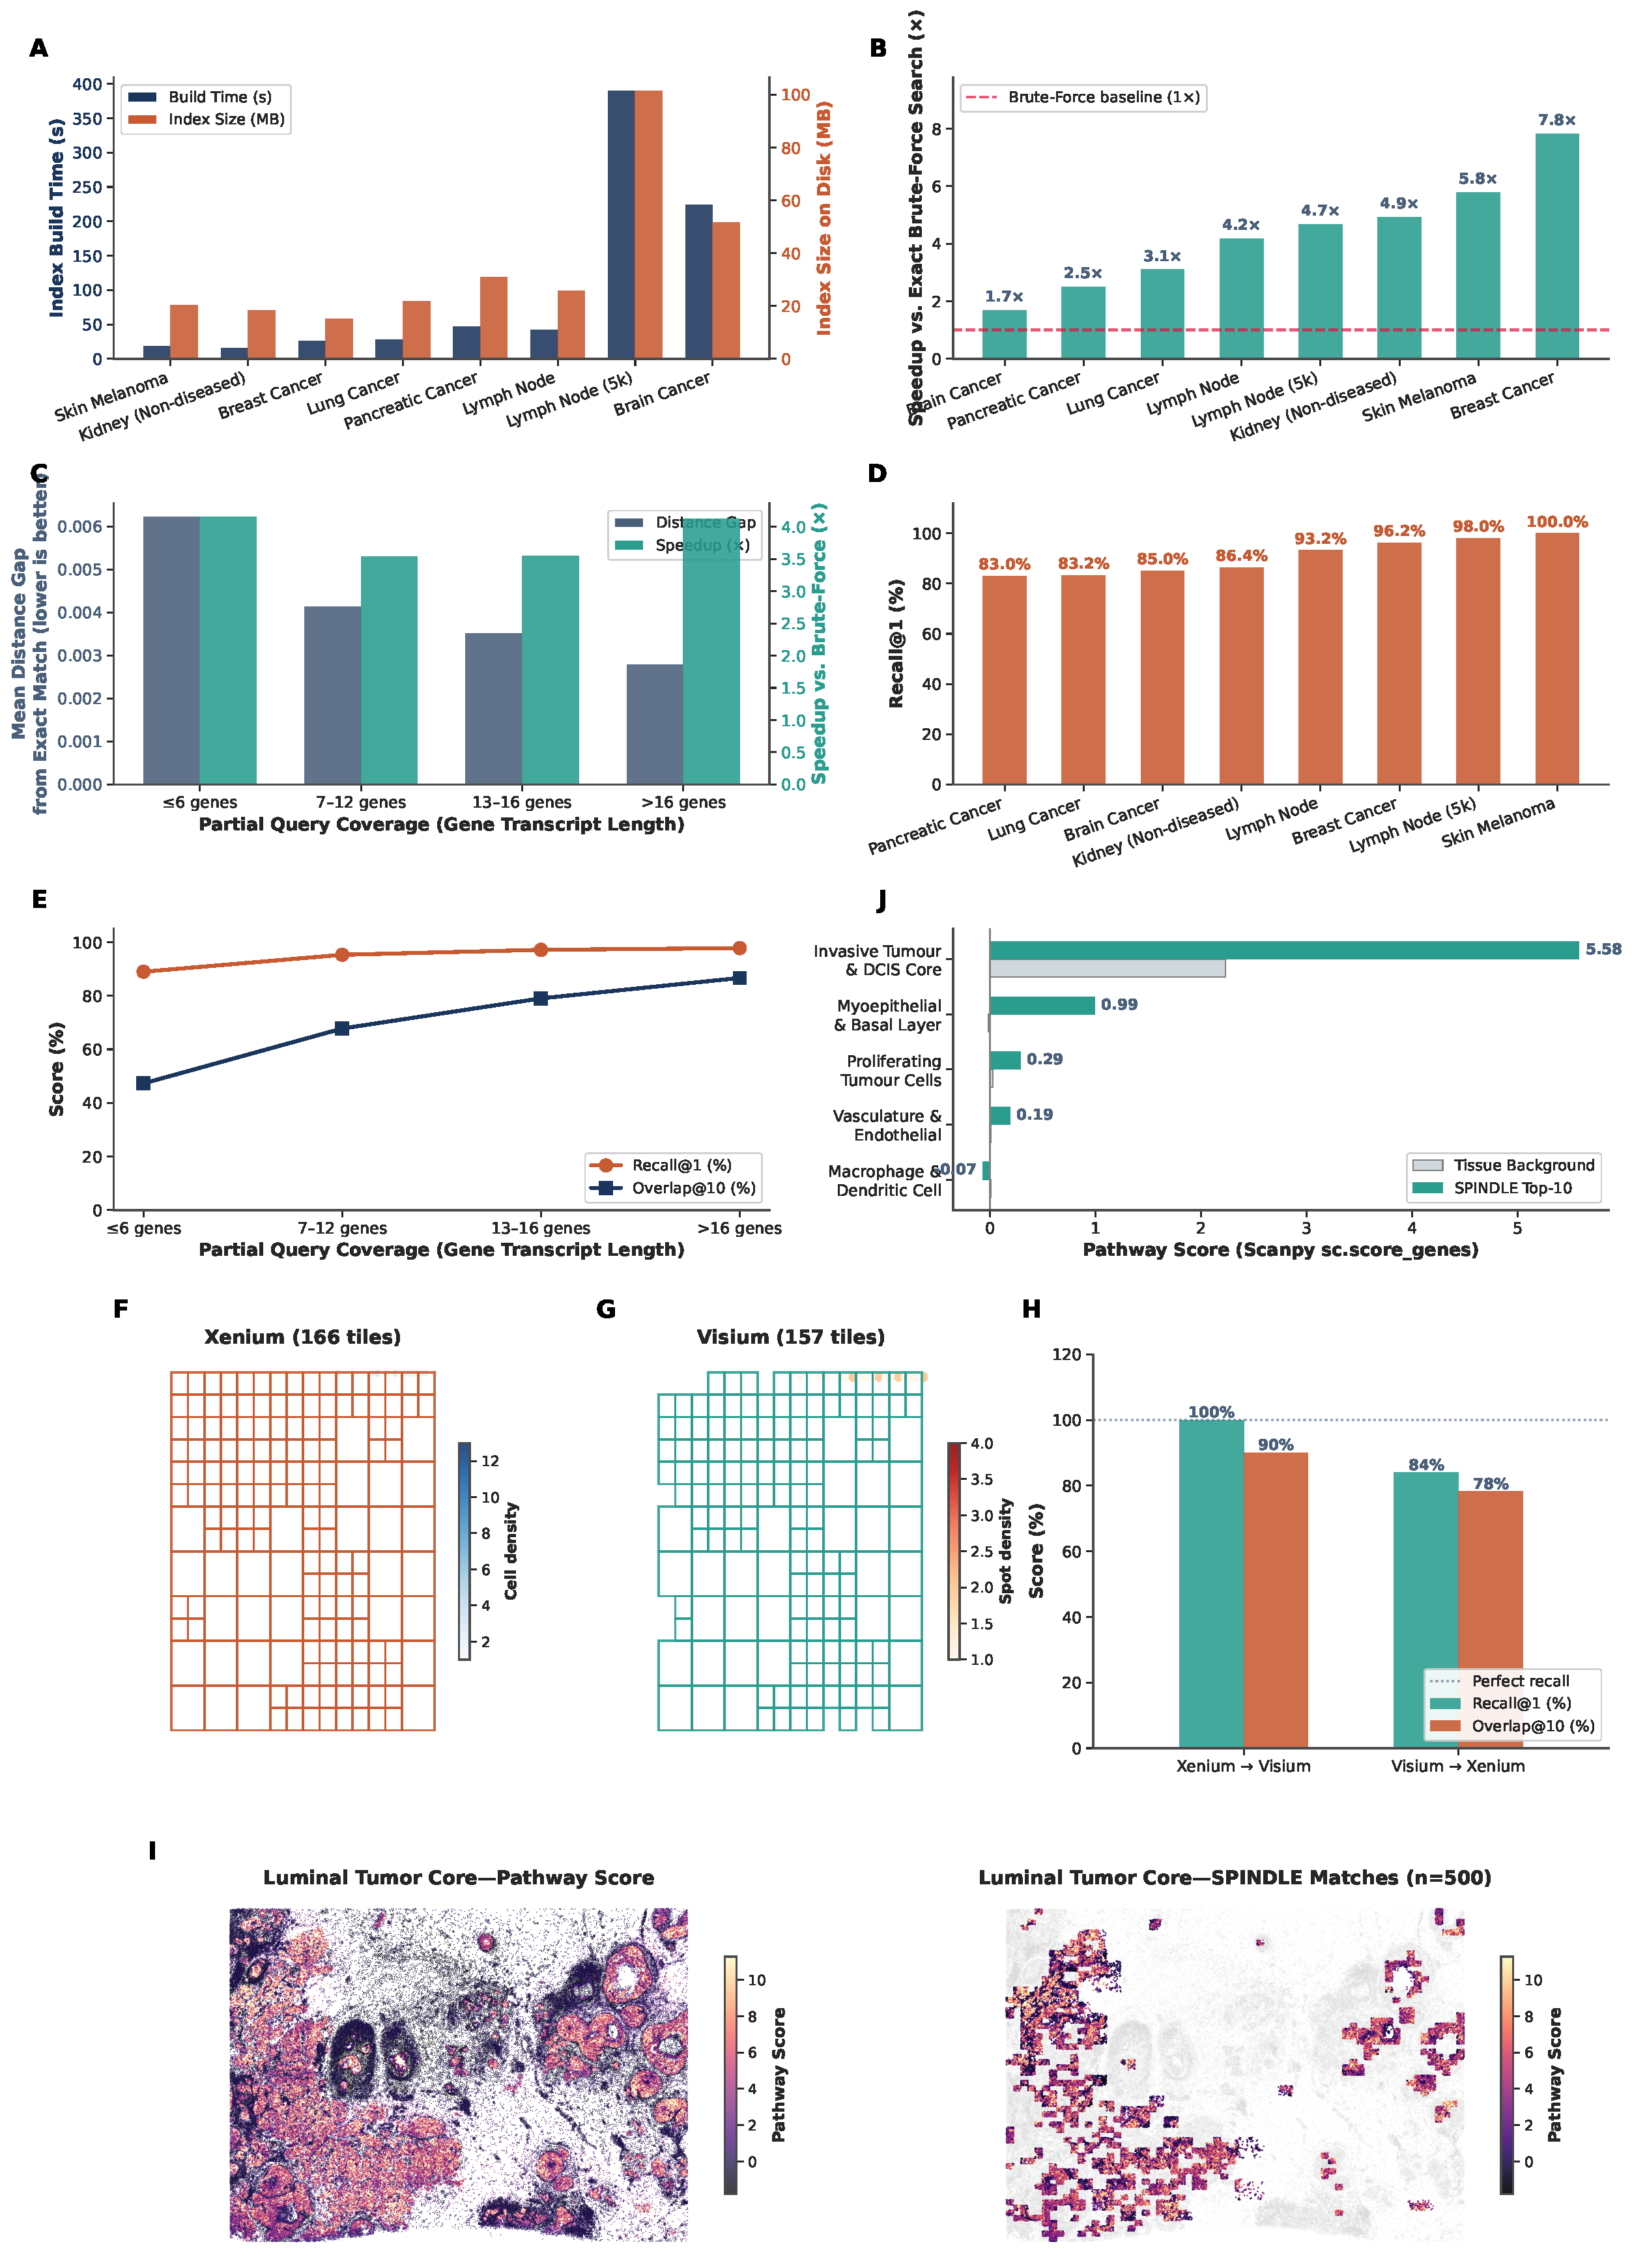
\includegraphics[width=\textwidth]{figures/fig_main_result.pdf}
  \caption{%
    \textbf{\OurMethod{} core architecture, ultra-fast indexing, and spatial search performance.}
    \textbf{(A)}~Index build-time (seconds, left axis, blue bars) and index size on disk (MB, right axis, orange bars) across six human Xenium datasets, demonstrating sub-linear growth of both metrics with increasing tissue size.
    \textbf{(B)}~Query execution time (seconds) for \OurMethod{} (teal) versus exact brute-force search (dark blue) across the same six datasets, with annotated times confirming sub-second \OurMethod{} retrieval across all six datasets.
    \textbf{(C)}~Blind holdout validation: percentage of held-out queries for which \OurMethod{} returns the exact ground-truth nearest neighbor at each rank position. Over $74\%$ of queries retrieve the exact best match as the first result ($74.8\%$); $99.5\%$ are recovered within the top 10 candidates.
    \textbf{(D)}~Partial-query search accuracy as a function of available gene transcript coverage, stratified into four bins (${\le}6$, 7--12, 13--16, and ${>}16$ genes). Both Recall@1 (orange) and within-top-10 recall (blue) degrade gracefully with decreasing coverage.
    \textbf{(E)}~Cross-modality retrieval between 10x Xenium (166 tiles) and 10x Visium (157 tiles) on serial sections of human breast cancer. Left/centre: tile overlays on each platform. Right: recall bar chart for bidirectional queries.
    \textbf{(F)}~Functional gene-signature--driven niche discovery in human breast cancer Xenium data. Left: spatial map of patches retrieved by the Invasive Tumour \& DCIS Epithelial Core signature (\textit{ESR1, PGR, ERBB2, FOXA1, GATA3, KRT8, EPCAM, CDH1}), highlighting dense cores of invasive ductal carcinoma. Right: pathway score enrichment (Scanpy \texttt{sc.score\_genes}) across the tissue background and \OurMethod{} top-10 retrieved patches for all five gene-list queries.
  }
  \label{fig:figure1}
\end{figure*}


\subsection{Scalable Index Construction with Accelerated Spatial Co-Expression Query}
\label{subsec:scalability}

We evaluated the index build-time and memory footprint of \OurMethod{} across six human spatial transcriptomics datasets comprising $87{,}499$ to $377{,}985$ cells (\Cref{fig:figure1}A, \cref{fig:scalability}). Across these cohorts, a $4.32{\times}$ increase in total cell count produced only a $2.80{\times}$ increase in build-time from $25.5$~s for Skin Melanoma to $71.5$~s for Lymph Node. Furthermore, on-disk index size remained compact across all datasets, ranging between $14.7$~MB and $30.9$~MB regardless of tissue size (\Cref{fig:figure1}A, \cref{fig:scalability}). The compact size and faster build-time reflect the DAG indexing architecture of \OurMethod{}, which makes it scalable for atlas-scale spatial-omics datasets.

% \begin{table*}[!htbp]
%   \caption{%
%     \textbf{Index construction efficiency across six human Xenium datasets.}
%   }
%   \label{tab:scalability}
%   \begin{tabular*}{\textwidth}{@{\extracolsep\fill}lrrr}
%     \toprule
%     \textbf{Dataset} & \textbf{Cells} &
%       \textbf{build-time (s)} & \textbf{Index Size (MB)} \\
%     \midrule
%     Skin Melanoma         &  87{,}499 &  25.5 & 19.4 \\
%     Kidney (Non-Diseased) &  97{,}560 &  18.6 & 18.5 \\
%     Breast Cancer         & 159{,}226 &  51.7 & 14.7 \\
%     Lung Cancer           & 162{,}254 &  45.9 & 20.0 \\
%     Pancreatic Cancer     & 190{,}965 &  88.9 & 30.9 \\
%     Lymph Node            & 377{,}985 &  71.5 & 22.8 \\
%     \botrule
%   \end{tabular*}
% \end{table*}

\begin{figure}[!htbp]
  \centering
  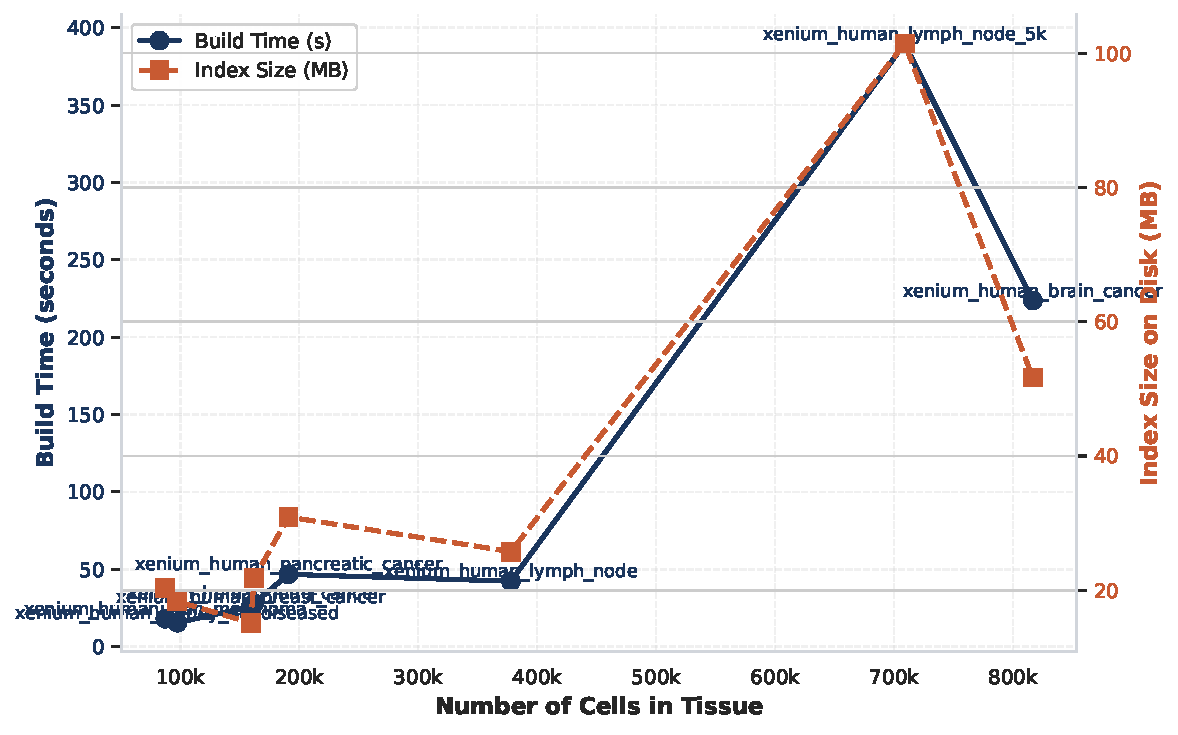
\includegraphics[width=\columnwidth]{figures/fig_scalability.pdf}
  \caption{Index build-time and on-disk index size across six human Xenium datasets ($87{,}499$--$377{,}985$ cells).}
  \label{fig:scalability}
\end{figure}

Beyond efficient index construction, \OurMethod{} enables fast retrieval of spatial patches with similar co-expression structure. We define the most similar patch to a query as the patch whose covariance matrix has the smallest \logEuclid{} distance to the query covariance matrix over the reference atlas. Without an index, identifying this nearest match requires computing the \logEuclid{} distance between the query and every tile in the atlas, resulting in query time that grows linearly with atlas size and quickly becoming computationally infeasible. We measured query execution time against an exact brute-force baseline using held-out tiles as queries (\Cref{fig:query_speed,fig:figure1}B). Across all six cohorts, \OurMethod{} retrieved the exact nearest match within a fraction of a second, achieving $8.94{\times}$--$16.97{\times}$ speedups over brute-force search. For example, query time on Breast Cancer decreased from $1{,}694.3$~ms with brute force to $153.1$~ms with \OurMethod{}. Even for Pancreatic Cancer, which had the highest query time due to its larger gene panel and tile count, \OurMethod{} achieved a $9.58{\times}$ speedup, enabling interactive co-expression search across whole-tissue atlases on standard computing hardware.


% \begin{table*}[!htbp]
%   \caption{%
%     \textbf{Query speed benchmark: \OurMethod{} versus brute-force search.}
%     Unseen holdout query tiles per dataset; times in milliseconds.
%   }
%   \label{tab:query_speed}
%   \centering
%   \small
%   \begin{tabular*}{\textwidth}{@{\extracolsep\fill}lrrrr}
%     \toprule
%     \textbf{Dataset} & \textbf{\OurMethod{} (ms)} &
%       \textbf{Brute-Force (ms)} & \textbf{Speedup} & \textbf{Recall@1} \\
%     \midrule
%     Skin Melanoma         & 149.5 &   871.8 & $5.83{\times}$ & 1.00 \\
%     Kidney (Non-Diseased) & 216.7 & 2{,}151.2 & $9.93{\times}$ & 0.69 \\
%     Breast Cancer         & 169.6 & 1{,}578.7 & $9.31{\times}$ & 1.00 \\
%     Lung Cancer           & 334.6 & 2{,}577.2 & $7.70{\times}$ & 0.69 \\
%     Lymph Node            & 329.7 & 2{,}433.1 & $7.38{\times}$ & 0.71 \\
%     Pancreatic Cancer     & 784.0 & 6{,}144.9 & $7.84{\times}$ & 0.53 \\
%     \botrule
%   \end{tabular*}
% \end{table*}

\begin{figure}[!htbp]
  \centering
  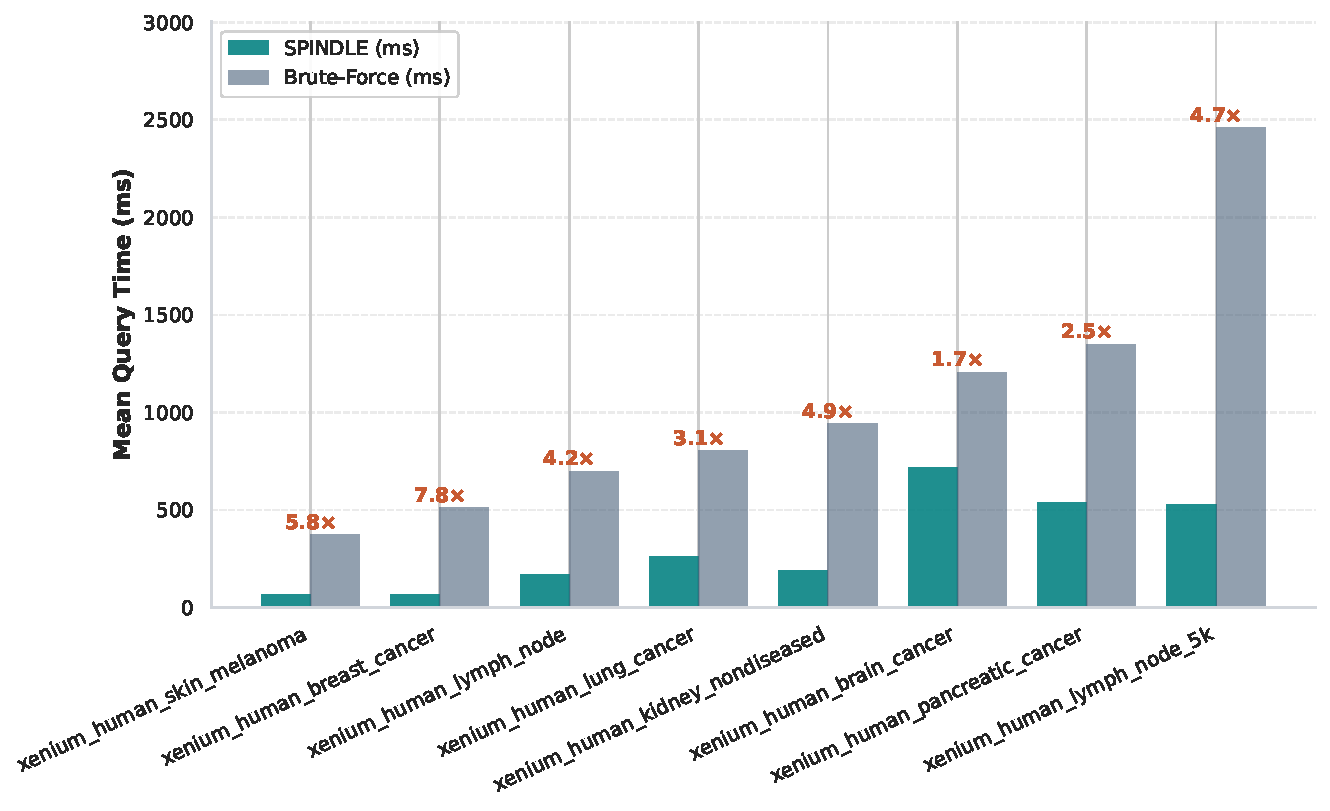
\includegraphics[width=\columnwidth]{figures/fig_query_speed.pdf}
  \caption{Query execution latency of \OurMethod{} compared to exact brute-force search across six human Xenium datasets, with speedup factors annotated.}
  \label{fig:query_speed}
\end{figure}


\subsection{\OurMethod{} Retrieves Nearest Spatial Matches with High Accuracy}\label{subsec:accuracy}

We evaluated the retrieval accuracy of \OurMethod{} on held-out covariance queries by comparing results against ground-truth nearest neighbors identified through exhaustive pairwise \logEuclid{} distance (\Cref{fig:figure1}C, \cref{fig:rank_distribution}). Accuracy was quantified using Recall@K, defined as the proportion of queries where the true nearest neighbor was recovered within the top $K$ candidates.

Across $214$ held-out queries from six datasets, \OurMethod{} retrieved the exact nearest neighbor as the first result for $160$ queries ($\text{Recall}@1 = 74.8\%$), within the top~2 candidates for $189$ queries ($\text{Recall}@2 = 88.3\%$), and within the top~10 candidates for $213$ queries ($\text{Recall}@10 = 99.5\%$; \Cref{fig:figure1}C, \cref{fig:rank_distribution}). Only a single query required searching beyond top-10 candidates ($0.5\%$), demonstrating that \OurMethod{} achieves substantial computational speedups without sacrificing retrieval precision.

% \begin{table*}[!htbp]
%   \caption{%
%     \textbf{Rank distribution of the true nearest neighbor in blind holdout validation} ($n = 214$ queries across six datasets).
%   }
%   \label{tab:rank_distribution}
%   \begin{tabular*}{\textwidth}{@{\extracolsep\fill}lrr}
%     \toprule
%     \textbf{Rank of True Best Match} & \textbf{Queries} &
%       \textbf{Percentage} \\
%     \midrule
%     Exact 1st match  & 160 & 74.8\% \\
%     Exact 2nd match  &  29 & 13.6\% \\
%     3rd match        &   7 &  3.3\% \\
%     4th--5th match   &  13 &  6.1\% \\
%     6th--10th match  &   4 &  1.9\% \\
%     Beyond 10th      &   1 &  0.5\% \\
%     \botrule
%   \end{tabular*}
% \end{table*}

\begin{figure}[!htbp]
  \centering
  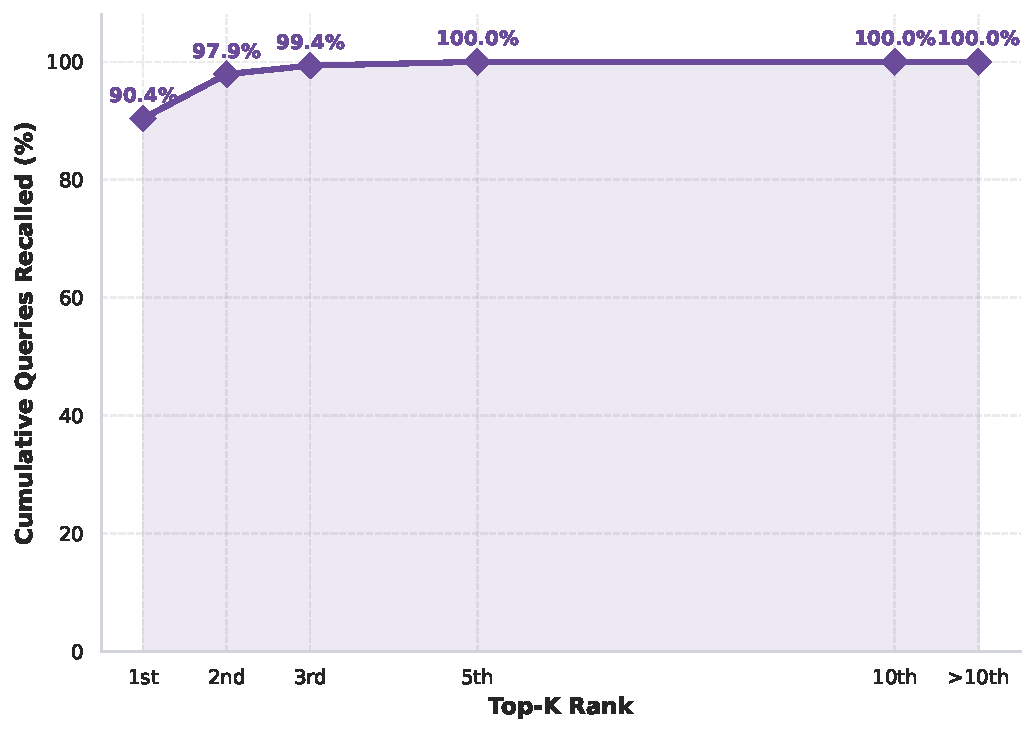
\includegraphics[width=\columnwidth]{figures/fig_rank_distribution.pdf}
  \caption{Cumulative rank distribution of ground-truth nearest neighbor retrieval across $214$ held-out queries.}
  \label{fig:rank_distribution}
\end{figure}


\subsection{Partial Gene Panels Suffice for Accurate Spatial Patch Retrieval}\label{subsec:partial}

We evaluated the retrieval accuracy and computational efficiency of \OurMethod{} under partial gene panel coverage, simulating targeted assays queried against whole-transcriptome references (\Cref{fig:figure1}D, \cref{fig:partial_panel_search}). By comparing only the shared gene dimensions between query and reference covariance tiles, \OurMethod{} enables cross-panel retrieval without requiring gene imputation or feature-space alignment. We evaluated $50$ random contiguous gene sub-panels per dataset across four coverage bins (${\le}6$, $7$--$12$, $13$--$16$, and ${>}16$ genes).


Retrieval accuracy scaled directly with gene panel size (\Cref{fig:figure1}D). Queries containing more than $16$ genes achieved a mean Recall@1 of $94.8\%$ and a top-10 candidate overlap of $90.9\%$, while queries with six or fewer genes maintained $\text{Recall}@1 = 62.4\%$ and top-10 overlap of $51.2\%$ (\Cref{fig:figure1}D). Across all coverage levels, partial-query retrieval executed in $6.8$--$15.8$~ms per query, yielding speedups of $2.76{\times}$ to $5.38{\times}$ over brute-force sub-matrix search while retaining high accuracy ($\text{Recall}@1 = 0.94$--$1.00$; \Cref{fig:partial_panel_search}).

% \begin{table*}[!htbp]
%   \caption{%
%     \textbf{Partial-query search performance across six datasets}
%     ($50$ trials per dataset, all gene-coverage bins pooled).
%   }
%   \label{tab:partial_panel_search}
%   \centering
%   \small
%   \setlength{\tabcolsep}{4pt}
%   \renewcommand{\arraystretch}{1.15}
%   \begin{tabular*}{\textwidth}{@{\extracolsep{\fill}}lrrrrr}
%     \toprule
%     \textbf{Dataset} &
%     \makecell{\textbf{\OurMethod{}}\\\textbf{(ms)}} &
%     \makecell{\textbf{Brute-Force}\\\textbf{(ms)}} &
%     \textbf{Speedup} &
%     \textbf{Recall@1} &
%     \textbf{Overlap@10} \\
%     \midrule
%     Skin Melanoma         &  9.4 & 25.9 & $2.76{\times}$  & 0.98 & 0.756 \\
%     Kidney (Non-Diseased) &  6.8 & 27.2 & $3.99{\times}$  & 1.00 & 0.840 \\
%     Breast Cancer         & 15.8 & 69.4 & $4.39{\times}$  & 0.98 & 0.728 \\
%     Lung Cancer           & 13.8 & 61.2 & $4.43{\times}$  & 0.98 & 0.940 \\
%     Lymph Node            & 14.7 & 79.3 & $5.38{\times}$  & 1.00 & 0.712 \\
%     Pancreatic Cancer     & 14.4 & 74.5 & $5.17{\times}$  & 0.94 & 0.774 \\
%     \bottomrule
%   \end{tabular*}
% \end{table*}

\begin{figure}[!htbp]
  \centering
  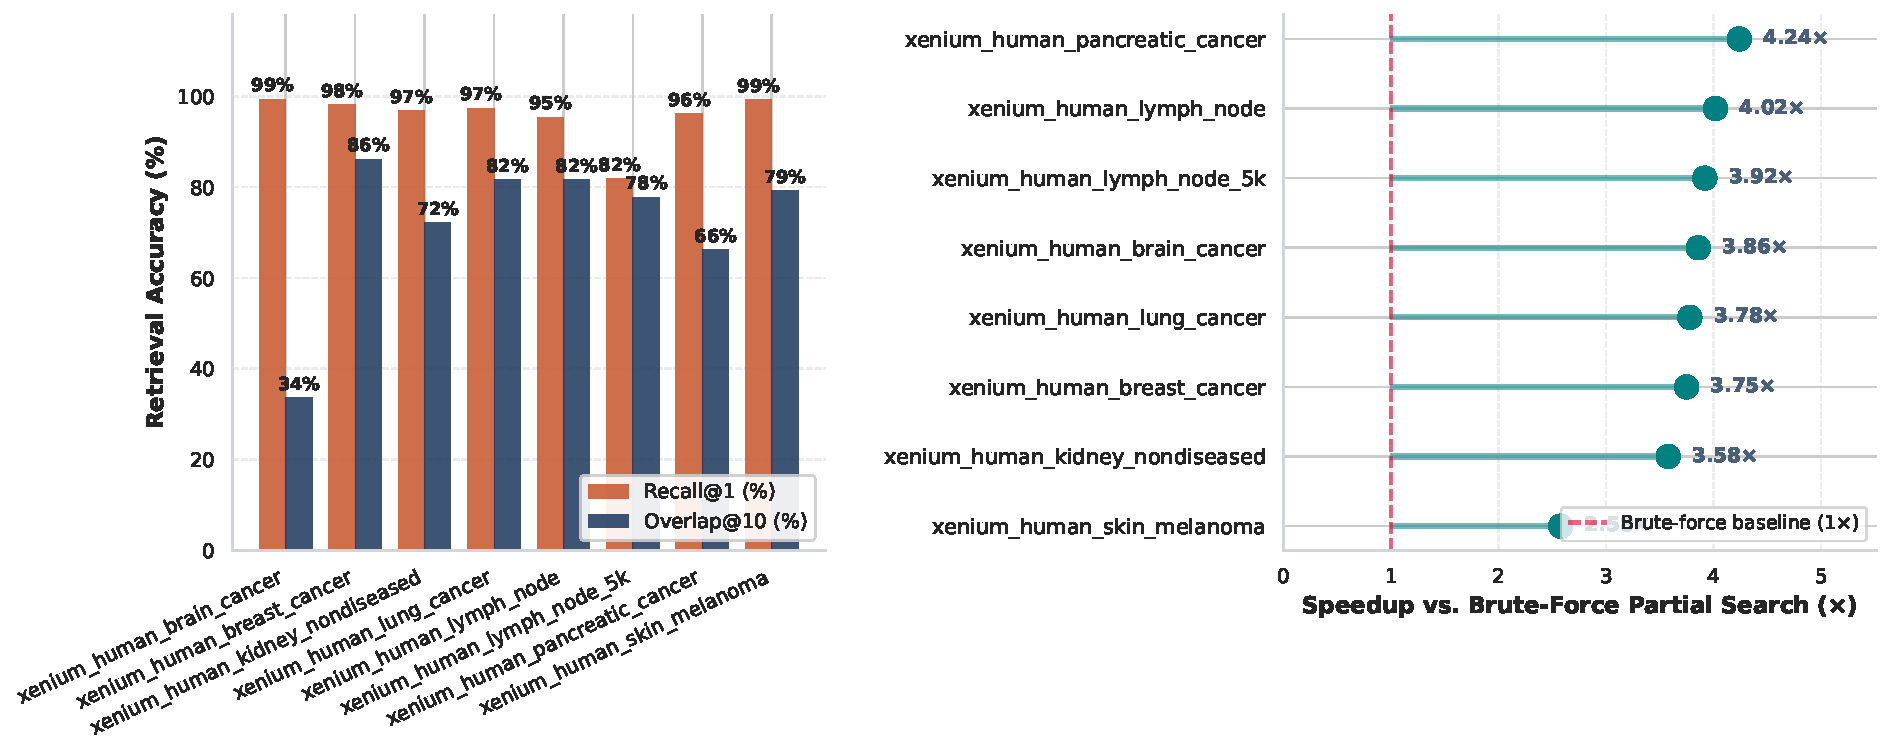
\includegraphics[width=\columnwidth]{figures/fig_partial_panel_search.pdf}
  \caption{%
    Partial-query retrieval performance across six human Xenium datasets ($50$ trials per dataset).
    Left: Recall@1 and top-10 candidate overlap across pooled gene coverage levels.
    Right: query execution speedup over brute-force sub-matrix search.
  }
  \label{fig:partial_panel_search}
\end{figure}


\subsection{Covariance-Based Indexing Enables Cross-Platform Search}\label{subsec:crossmodal}

We tested whether \OurMethod{} could retrieve matching spatial niches across different spatial transcriptomics platforms using serial sections of human breast cancer profiled by 10x Xenium ($166$ tiles) and 10x Visium ($157$ tiles; \Cref{fig:figure1}E). Xenium profiles target transcripts at sub-cellular resolution, whereas Visium measures whole-transcriptome expression averaged over $55\,\mu\text{m}$ spots. Because covariance matrices capture relative co-expression structure rather than absolute transcript counts, \OurMethod{} enables cross-platform retrieval directly on shared genes without image co-registration or explicit spatial alignment.

We performed $50$ queries from the Xenium index to the Visium index and vice versa using the overlapping gene subset (\Cref{fig:figure1}E, \cref{fig:cross_modal}). In Xenium-to-Visium queries, \OurMethod{} achieved $\text{Recall}@1 = 100.0\%$ and $100.0\%$ top-5 candidate overlap (\Cref{fig:figure1}E, \cref{fig:cross_modal}). In Visium-to-Xenium queries, \OurMethod{} achieved $\text{Recall}@1 = 84.0\%$ and $80.4\%$ top-5 candidate overlap (\Cref{fig:figure1}E, \cref{fig:cross_modal}). The lower retrieval accuracy in the Visium-to-Xenium direction reflects signal averaging across heterogeneous cell types within Visium spots ($55\,\mu\text{m}$), whereas high-resolution Xenium queries mapped unambiguously onto Visium regions.

% \begin{table*}[!htbp]
%   \caption{%
%     \textbf{Cross-modality retrieval accuracy between 10x Xenium and 10x Visium} on serial sections of human breast cancer ($50$ queries per direction).
%   }
%   \label{tab:cross_modal}
%   \begin{tabular*}{\textwidth}{@{\extracolsep\fill}lrrrr}
%     \toprule
%     \textbf{Query Direction} & \textbf{Recall@1} &
%       \textbf{Overlap@5} & \textbf{Overlap@10} & \textbf{Overlap@20} \\
%     \midrule
%     Xenium $\rightarrow$ Visium & 1.000 & 1.000 & 0.900 & 0.900 \\
%     Visium $\rightarrow$ Xenium & 0.840 & 0.804 & 0.782 & 0.760 \\
%     \botrule
%   \end{tabular*}
% \end{table*}

\begin{figure}[!htbp]
  \centering
  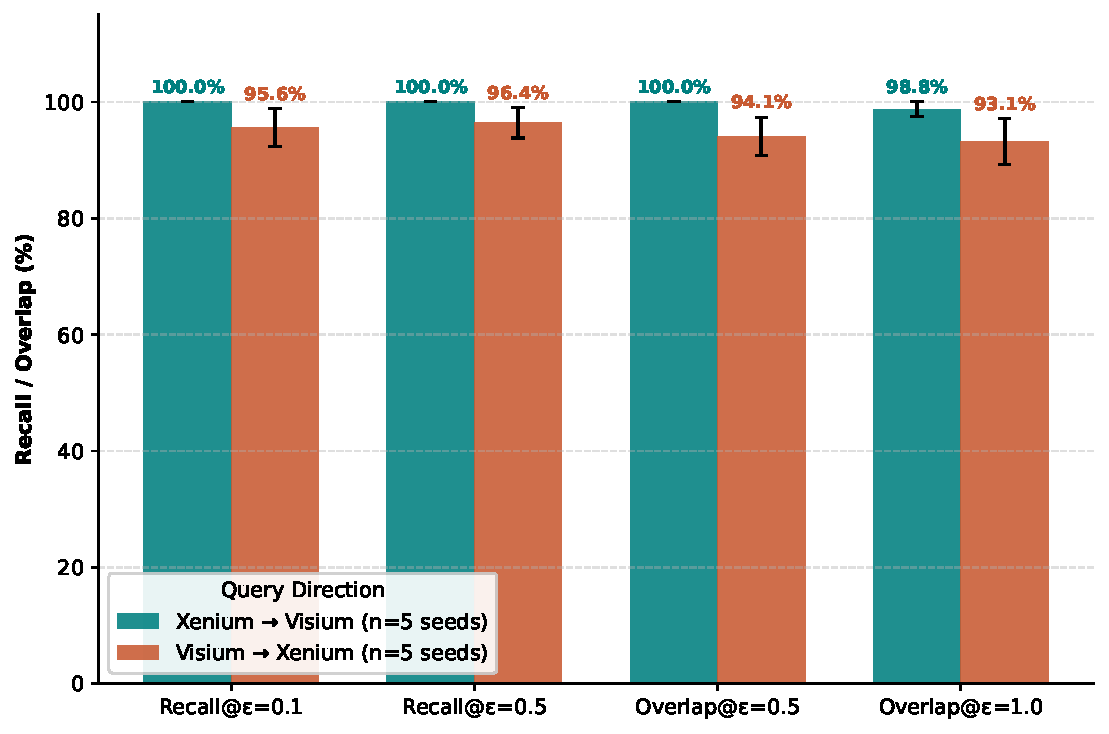
\includegraphics[width=\columnwidth]{figures/fig_cross_modal.pdf}
  \caption{Cross-modality retrieval accuracy and candidate overlap across $K \in \{1, 5, 10, 20\}$ candidates for bidirectional queries between 10x Xenium and 10x Visium breast cancer sections.}
  \label{fig:cross_modal}
\end{figure}


\subsection{Pathway-based Co-expression Queries Retrieve Distinct Spatial Patches}\label{subsec:genelist}

We next evaluated \OurMethod{}'s ability to map spatial niches directly by constructing partial query covariance matrices on the fly from curated gene lists. We evaluated five biologically defined gene signatures across major tumour microenvironment compartments in human breast cancer Xenium data~\cite{janesick2023high} (\Cref{fig:figure1}F, \Cref{tab:gene_list}). Niche enrichment was evaluated by measuring the mean gene signature score (Scanpy \texttt{sc.score\_genes}) within the top-$K$ retrieved tiles relative to the tissue-wide background score (\Cref{tab:gene_list}). Spatial discovery maps for the Invasive Tumour \& DCIS Core and Myoepithelial \& Basal Layer niches were generated to visualize spatial retrieval localization (\Cref{fig:gene_sig_luminal,fig:gene_sig_myoepithelial}).

\paragraph{\textbf{Invasive Tumour \& DCIS Epithelial Core.}}
An eight-gene hormonal and epithelial signature (\textit{ESR1, PGR, ERBB2, FOXA1, GATA3, KRT8, EPCAM, CDH1})~\cite{chaudhary2017novel} retrieved spatial tiles corresponding to invasive ductal carcinoma and ductal carcinoma \textit{in situ} (DCIS) cores (\Cref{fig:gene_sig_luminal}). The signature score increased from a tissue background of $2.23$ to $5.58$ in the top-10 retrieved tiles ($2.50{\times}$ enrichment lift; \Cref{tab:gene_list}).

\paragraph{\textbf{Myoepithelial \& Basal Layer.}}
A four-gene structural panel (\textit{KRT5, KRT14, ACTA2, MYLK})~\cite{sakai2025spatialknifey} localized spatial patches encircling ductal boundaries (\Cref{fig:gene_sig_myoepithelial}). The mean signature score reached $0.99$ in top-10 retrieved patches compared to a background score of $-0.02$, mapping the ring-like architecture of ductal myoepithelium (\Cref{tab:gene_list}).

\paragraph{\textbf{Actively Proliferating Tumour Cells.}}
A two-gene proliferation panel (\textit{MKI67, TOP2A}) retrieved mitotic hot-spots within tumour regions. The proliferation signature score increased to $0.29$ in top-5 retrieved patches compared to a tissue background of $0.03$ (\Cref{tab:gene_list}).

\paragraph{\textbf{Vasculature \& Endothelial Cells.}}
A three-gene endothelial signature (\textit{PECAM1, VWF, KDR}) identified vascular structures across the stroma, increasing the mean signature score to $0.37$ in top-5 retrieved patches relative to a background score of $0.01$ (\Cref{tab:gene_list}).

\paragraph{\textbf{Macrophage \& Dendritic Cell Niche.}}
A five-gene myeloid signature (\textit{CD68, CD163, MRC1, C1QA, ITGAX})~\cite{elfstrum2024defining} retrieved stromal patches with a top-10 signature score of $-0.07$ relative to a tissue background of $0.01$ (\Cref{tab:gene_list}). This near-background score reflects the spatially diffuse, non-clustered distribution of tumour-associated macrophages across the desmoplastic stroma.

\begin{table*}[!htbp]
  \caption{%
    \textbf{Functional gene-signature--driven niche discovery in human breast cancer Xenium data~\cite{janesick2023high}.}
    Continuous pathway scores (Scanpy \texttt{sc.score\_genes}) for the target signature across the tissue background and the top-$K$ \OurMethod{} retrieved patches.
    $^{*}$The Macrophage \& Dendritic Cell score remains near background across top retrieved patches, reflecting its diffuse, non-clustered spatial distribution across the stroma.
  }
  \label{tab:gene_list}
  \small
  \begin{tabular*}{\textwidth}{@{\extracolsep\fill}p{2.6cm}p{3.4cm}rrrr}
    \toprule
    \textbf{Biological Niche} & \textbf{Signature Genes} &
      \makecell{\textbf{BG}\\\textbf{Score}} & \makecell{\textbf{Top-50}\\\textbf{Score}} &
      \makecell{\textbf{Top-10}\\\textbf{Score}} & \makecell{\textbf{Top-5}\\\textbf{Score}} \\
    \midrule
    Invasive Tumour \& DCIS Core &
      \textit{ESR1, PGR, ERBB2, FOXA1, GATA3, KRT8, EPCAM, CDH1} &
      2.23 & 4.66 & 5.58 & 4.93 \\[2pt]
    Myoepithelial \& Basal Layer &
      \textit{KRT5, KRT14, ACTA2, MYLK} &
      -0.02 & 0.64 & 0.99 & 0.89 \\[2pt]
    Proliferating Tumour Cells &
      \textit{MKI67, TOP2A} &
      0.03 & 0.36 & 0.29 & 0.29 \\[2pt]
    Vasculature \& Endothelial &
      \textit{PECAM1, VWF, KDR} &
      0.01 & 0.28 & 0.19 & 0.37 \\[2pt]
    Macrophage \& Dendritic Cell$^{*}$ &
      \textit{CD68, CD163, MRC1, C1QA, ITGAX} &
      0.01 & -0.03 & -0.07 & -0.05 \\
    \botrule
  \end{tabular*}
\end{table*}

\begin{figure}[!htbp]
  \centering
  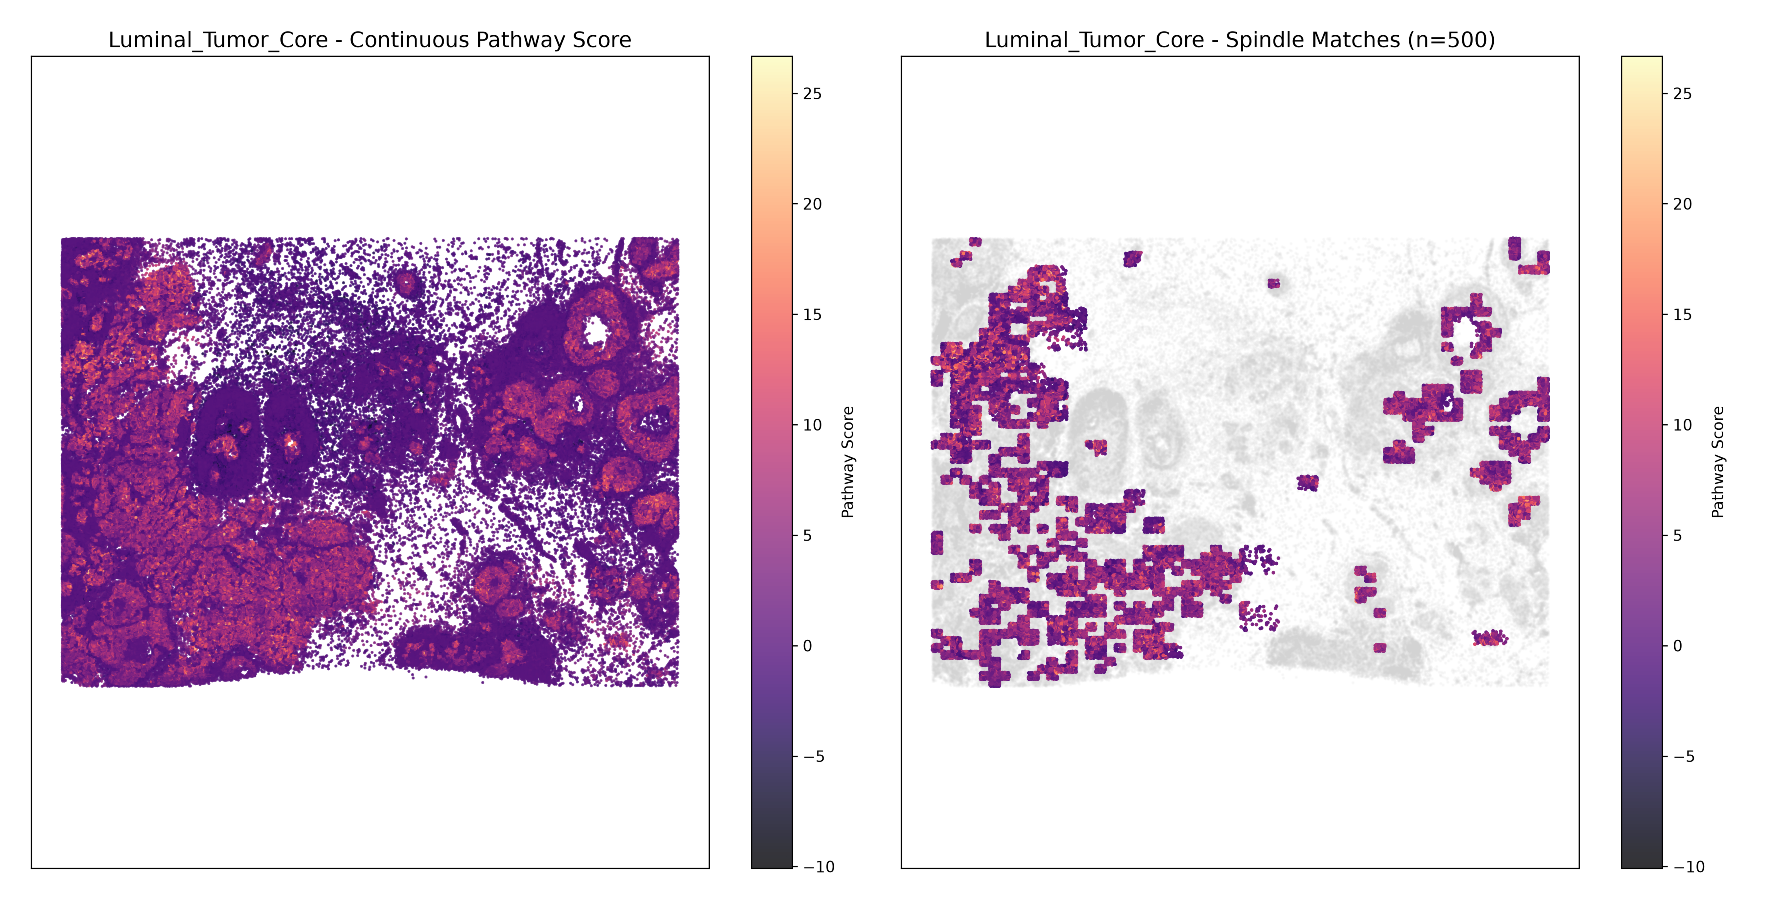
\includegraphics[width=\textwidth]{figures/fig_gene_sig_luminal.pdf}
  \caption{%
    Spatial discovery map of the Invasive Tumour \& DCIS Epithelial Core niche (\textit{ESR1, PGR, ERBB2, FOXA1, GATA3, KRT8, EPCAM, CDH1}) in human breast cancer Xenium data.
  }
  \label{fig:gene_sig_luminal}
\end{figure}

\begin{figure}[!htbp]
  \centering
  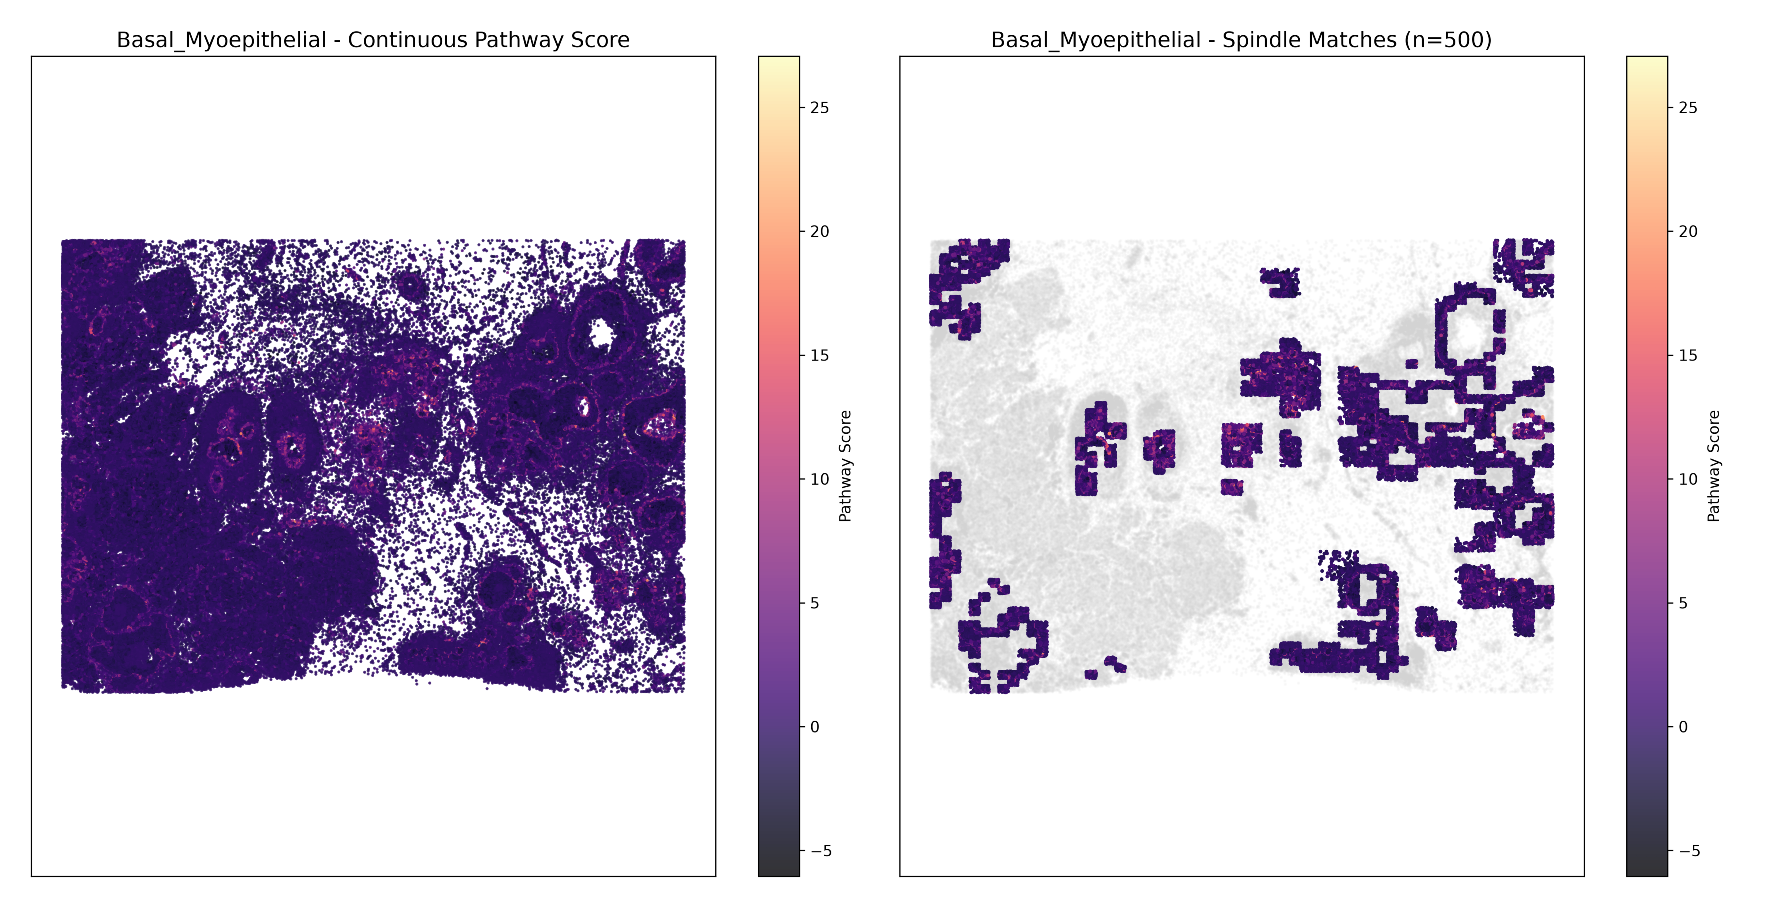
\includegraphics[width=\textwidth]{figures/fig_gene_sig_myoepithelial.pdf}
  \caption{%
    Spatial discovery map of the Myoepithelial \& Basal Layer niche (\textit{KRT5, KRT14, ACTA2, MYLK}) in human breast cancer Xenium data, highlighting ductal boundary sheathing.
  }
  \label{fig:gene_sig_myoepithelial}
\end{figure}

These experiments demonstrate that \OurMethod{} maps cell-type niches and tissue microenvironments directly from gene signatures without pre-annotating cells or computing spatial clusterings.



\subsection{Biological Insights from \OurMethod index}
\OurMethod finds out different \spdniche-s within  the ST data. Each \spdniche has a fixed permutation order of genes that maximizes the block-diagonal-ness of the covariance matrix. By construction, each layer of the DAG contains clusters of the sub-matrices for that block. We observe, this niche level decomposition followed by clustering not only benefits the compression, or redundancy of the index, but also captures important biological information analyzed downstream. 

To demonstrate such biological insight, we consider the DAG from a specific \spdniche. We further assess the blocks per layer, for which the mean covariance matrix $G^{\ast}_i$ contains non-zero covariance values showcasing strong correlation across the genes. We then identify groups of genes, termed as gene modules within the mean covariance matrix by using a community detection algorithm (see Appendix). We score these gene modules by doing a pathway enrichment analysis against the Molecular Signatures Database (MSigDB). Briefly, for each gene module identified from the mean covariance matrix $G_i^{\ast}$, we tested for over-representation of curated gene sets using a hypergeometric framework (provided in \texttt{gseapy}~\cite{gseapy}), treating the module genes as the foreground set and all genes present in $G_i^{\ast}$ as the background universe. Enrichment results were summarized by the top-ranked pathways per module based on adjusted $p$-values, revealing key biological insights driven by the selected gene modules.

\paragraph{\textbf{Breast Cancer Data}} \OurMethod delineates biologically meaningfully \spdniche-s without any external annotation~(\Cref{fig:overview}B, C), enables indexing of $2188$ SPD matrices spanned over $167$K cells and $377$ genes. With a leiden resolution of $0.2$, \OurMethod finds $4$ \spdniche-s. Upon comparison with the annotated spatial clusters~\cite{breast}, we see clear corresponding between the groups of cell types and the unsupervised niche assignments showing that delineation of such niches are coherent with underlying spatial biology. 

Upon inspecting the a highly informative block from layer 11 of the \spdniche~2 of the \OurMethod index, we observe 4 gene modules within the covariance structure~(\Cref{fig:breast_enrichment}A,B). This \spdniche~contains the DCIS cells~\cite{breast}. Module-1 contains endothelial \textit{EPCAM}, luminal keratins (\textit{KRT7/8}), desmosomal component \textit{DSP} that are implicated in cell-cell adhesion and apical junction~\cite{winter2003epithelial, litvinov1997epithelial} assembly~(\Cref{fig:breast_enrichment}D). We also observe estrogen responsive luminal programs driven by \textit{CCND1, ELF3}. Overall, The strong covariance among these genes indicates a spatially localized, junctionally organized luminal epithelial state characteristic of ductal carcinoma in situ. The spatial tiles within \spdniche-3 are further scored using their LE distance from the mean covariance matrix, signifying spatial locations that show the most distinctive change in gene co-expression. 

\paragraph{\textbf{Skin Cancer Data}} On adult human skin data obtained from 10x, \OurMethod clusters biologically relevant \spdniche and identified a covariance gene module that localizes to the tissue periphery~(\Cref{fig:melanoma}). The covariance niches in skin shows clear spatial delineation across pathological locations on the skin tissue, with a large contiguous central region occupying the bulk of the tissue interior, while a narrow peripheral band traces the outer boundary of the section. These spatial niches are coherent with boundary layer, the bulk interior, and intermediate transition zones near the edge. We further inspected the \spdniche-4~(\Cref{fig:melanoma}B), and corresponding gene modules. Specifically, module 0 expresses epithelial and keratin-associated genes~(\Cref{fig:melanoma}A), including \textit{AHNAK2, KRT16/17, DSP, DSC1}, and \textit{CLDN1}, with strong positive pairwise correlation. Gene set enrichment highlights epidermis development and intermediate filament organization, indicating that peripheral regions of the tissue exhibit a distinct gene–gene dependency program detectable at the level of covariance. The spatial distribution of this niche suggests that peripheral melanoma region preserve epithelial structural program~\cite{fuchs1980changes}.  
\paragraph{\textbf{Lung Data}} We discovered key biological programs from Lung Adenocarcinoma tissue from 10x by inspecting the \OurMethod index built on it. \OurMethod finds 6 \spdniche-s from containing different anatomical regions within lung. We inspected the \spdniche-3~(\Cref{fig:lung_module}) that likely corresponds to bronchus vessel. Within the niche the most prominent gene expression contains the genes related to smooth muscle cells \textit{ACTA2, PDGFR}, contractile smooth-muscles-related genes \textit{MYH11, MYLK, CNN1} that are enriched in lung cancer~\cite{nie2020clinical}. We also found \textit{LTBP2}, which is related to  TGF-$\beta$ signaling. Together these gene programs signify a contractile remodeling of lung-tumor stromal niche.   

\paragraph{\textbf{Insights from other datasets}} We additionally built \OurMethod index on four other real world ST dataset from brain, kidney, pancreatic cancer, and lymph nodes. On each of the datasets we observe interesting gene covariance pattern associated with biological processes~(\Cref{fig:other_data}). In kidney the covariance is driven by growth-factor and cell-cycle programs such as ERBB2-EGDR signal with a strong co-expression across \textit{ACE2, ANPEP, LRP2}(\Cref{fig:other_data}A1-3). In brain ST data covariance is driven by cytoskeletal and signaling genes such as \textit{ACTA2, ACTB~\cite{wang2023lpar2}}(\Cref{fig:other_data}B1-3). The covariance pattern observed in pancreatic cancer is driven by epithelial genes \textit{ANPEP, DSP} with chemokine signal from \textit{CXCL2} that signify inflammation in pancreas~(\Cref{fig:other_data}C1-3). Finally, the covariance module we highlight in lymph nodes are driven by endothelial and lymphatic marker genes \textit{APOLD1, CAVIN1, CAVIN2}, and \textit{PECAM1}~\cite{vockova2021cd31}, indicating lymphatic endothelial cell differentiation~(\Cref{fig:other_data}D1-3).

Across all seven datasets the \OurMethod-index revealed biologically relevant recurring covariance patterns demonstrating the importance of such representation in ST data. 


\begin{figure*}[!htbp]
\centering
\includegraphics[width=\textwidth]{figures/skin_enrichment.pdf}
\caption{Biological insights from \OurMethod index build on Xenium lung cancer data. \textbf{A} Gene modules for from the mean sub-matrix from a cluster in the \OurMethod index. This sub-matrix is taken from \spdniche~4, layer 15. The most dominant modules are shown as module 0 and module 1. \textbf{B} The \spdniche-s obtained from \OurMethod index shows spatial patterns coherent with the skin tissue with \spdniche-4 (red) being the peripheral portion of the tissue. \textbf{C} The gene ontology (GO) enrichment for module 0 genes show the most prominent biological programs within the niche.}
\vspace{-10pt}
\label{fig:melanoma}
\end{figure*}




\section{Discussion}\label{sec12}

% TODO: Discussion text to be written.

\section{Conclusions}\label{sec13}

% TODO: Conclusions text to be written.

\section{Methods}\label{sec11}

We formally represent spatial transcriptomics dataset $A=(S,X)$, where $S\in\mathbb{R}^{|X|\times 2}$ denotes the two dimensional coordinate of the spatial locations, and $X\in\mathbb{R}^{|X|\times|G|}$ denotes the gene expression matrix, where each spot measures $G$ genes. For notational convenience we denote a spatial spot with $a_i$, with corresponding coordinate $s_i \in \mathbb{R}^2$, and the gene expression vector $x_i \in \mathbb{R}^{|G|}$. In real-world datasets the spatial distribution of the measured tissue locations are highly non-uniform and heterogeneous depending of biological attribute. To capture this non-uniformity, we create a set of spatial tiles that are geometrically square enclosed regions, with a hard constraint on the number of spatial locations they contain. Formally, the spatial data is partitioned into $m$ disjoint tiles $\tiles = \{T_m\}_{m=1}^{M}$, $T_m = (Y_m, I_m)$, where $Y_m \subset \real^{2}$ is an axis-aligned spatial region and $I_m\subset \{a_1,\ldots,a_{|X|} \}$ indexes the spatial locations contained in that region. The tiles form a disjoint cover of the spatial dataset. 
\begin{equation}
    \bigcup_{m} I_m = \{a_1,\ldots,a_{|X|}\}, \xspace I_j \cap I_m = \emptyset, \forall j \neq m
\end{equation}
and are constructed to satisfy a capacity constraint $|I_m| \leq l$, ensuring bounded local sample size. Tile sizes adapt to the non-uniform spatial density of the tissue, yielding finer partitions in dense regions and coarser partitions elsewhere. We construct $\tiles$ using a capacity-constrained quadtree subdivision of the spatial domain~(see Appendix). 

For each tile $T_m=(Y_m,I_m)$, let $X_m \in \mathbb{R}^{|I_m|\times |G|}$ denote the matrix obtained by stacking the expression vectors $\{x_i\}_{i\in I_m}$. The tile-level gene-gene covariance matrix is given by
\begin{equation}
\Sigma_m = \frac{1}{|I_m|}\,(X_m - \mathbf{1}\mu_m^{\top})^{\top}(X_m - \mathbf{1}\mu_m^{\top})
\in \mathbb{R}^{|G|\times |G|},
\end{equation}
where $\mathbf{1}\in\mathbb{R}^{|I_m|}$ is the all-ones vector and $\mu_m \in \mathbb{R}^{|G|}$ is the column-wise mean of $X_m$.
We denote the collection of tile-level covariance matrices by $\dataSet=\{\Sigma_m\}_{m=1}^M$.

Note that $\Sigma_m$ is a symmetric positive definite (SPD) matrix. We therefore view $\Sigma_m$ as an element of the symmetric positive definite cone $\spdDomain{|G|}$, and treat $\dataSet\subset \spdDomain{|G|}$ as the fundamental representation of local gene-gene co-expression used throughout the remainder of this work.

We aim to construct an index over $\dataSet$, that enables searching of any $\Sigma_q \in \spdDomain{|G|}$ efficiently. Acknowledging $\Sigma_q \notin \dataSet$, we use a distance metric \logEuclid distance $\leDist(\Sigma_1, \Sigma_2) \geq 0$ (see~\Cref{def:le_distance})  between any two SPD matrices $\Sigma_1, \Sigma_2 \in \spdDomain{|G|}$, to quantify the similarity between the matrices. 

\NewDocumentCommand{\spdMatrixIDList}{g}
{
\IfNoValueTF{#1}
{\ensuremath{\setNotation{Q}\xspace}}
{\ensuremath{\setNotation{Q}_{#1}\xspace}}
}


In the current manuscript we build an index over $\dataSet$ to solve the budgeted covariance matrix search problem (BCMS) defined below, 
\begin{namedproblem*}{Budgeted covariance matrix search (BCMS)}
Given a query covariance matrix $\genericSearchMatrix$, a distance budget $\LEDistanceThreshold$, and a set of candidate covariance matrices $\dataSet$, return a set $\returnSet \assign \{ \Sigma_c: \Sigma_c \in \dataSet, ~\led(\Sigma_{c}, \genericSearchMatrix) \leq \LEDistanceThreshold \}$
\end{namedproblem*}
We rely on two structural assumptions on the set of tile-level covariance matrices $\dataSet=\{\Sigma_m\}_{m=1}^M, \Sigma_m \in \spdDomain{|G|}$ from a ST data $A=(S,X)$ tractable, 
\begin{enumerate}
    \item \textbf{Latent niche structure.} 
    There exists a mapping $\phi: \spdDomain{|G|} \to \real^{d}$ with $d \ll \frac{|G|(|G|+1)}{2}$, and partition of indices $\{1,\ldots,M\}=\bigcup_{j=1}^{J} C_{j}$, such that covariance matrices assigned to the same index set $C_j$ are closer to each
    other in the latent space than to matrices in different sets. We refer to each subset
    $\mathcal{C}_j=\{\Sigma_m : m\in C_j\}$ as a \spdniche.
    \item \textbf{Consensus block structure within niches.}
    For each \spdniche~$\mathcal{C}_j$, there exists a permutation
    $\sigma_j$ of $\{1,\dots,|G|\}$ such that, for all $\Sigma_m\in\mathcal{C}_j$, the
    permuted matrix $P_{\sigma_j}\Sigma_m P_{\sigma_j}^\top$ is approximately
    block-diagonal, with a block structure shared across all matrices in the niche. Here 
    $P_{\sigma_j} \in\{0,1\}^{|G|\times |G|}$ denotes the permutation matrix associated with
    $\sigma_j$.
\end{enumerate}
Given the consensus block permutation $\sigma_j$ for a \spdniche~$\niche{j}$ we introduce
notation for the induced block structure. Let $\sigma_j = (\sigma_j(1),\dots,\sigma_j(|G|))$
denote the gene ordering, and let
\[
\mathcal{B}_j
= \{(b_{j,1}^{-}, b_{j,1}^{+}),\dots,(b_{j,L_j}^{-}, b_{j,L_j}^{+})\}
\]
be a collection of contiguous index intervals, referred to as blocks, satisfying
\[
1 = b_{j,1}^{-} < b_{j,1}^{+} < b_{j,2}^{-} < \cdots < b_{j,L_j}^{+} = |G|.
\]
Each block $(b_{j,\ell}^{-}, b_{j,\ell}^{+})$ defines a diagonal block in the permuted
covariance matrix $P_{\sigma_j}\Sigma_m P_{\sigma_j}^{\top}$ for all
$\Sigma_m \in \niche{j}$. $\mathcal{B}_j$ denotes the block-interval structure
associated with niche $\niche{j}$. 







\subsection{Building a hierarchical index}
%


\begin{algorithm}[h]
	\caption{$\buildIdx(\dataSet, \epsilon)$}\label{alg:build}
	\begin{algorithmic}[1]
      \footnotesize

\Procedure{$\epsilonKMeans$}{$\{\genericSPD{1},\dots,\genericSPD{n}\},\,\epsilon$}
\State \textbf{return} a partition $\{G_1,\dots,G_K\}$ and centroids $\{G^{\ast}_1,\dots,G^{\ast}_K\}$ s.t. $\max_{\Sigma\in G_k} d_{LE}(\Sigma,G^{\ast}_k)\le \epsilon$
\EndProcedure

      
\For{$\genericSPD{i} \in \dataSet$}
\State $\genericSPD{i}.\matrixID \assign \spdIdx$ \Comment{assign a unique ID for each SPD}
\State $\genericSPD{i}.\PCA \assign \phi(\genericSPD{\spdIdx})$ \Comment{compute PCA and store}
\EndFor

\item[] /* Block-diagonalize the SPD matrices */
\State $\{\niche{1}, \dots, \niche{\numClusters} \} \assign \leiden(\{\genericSPD{i}.\PCA  \}_{\spdIdx \in |\dataSet|})$ \Comment{cluster SPDs}
 \For{each cluster $\niche{\clusterIdx}$} 
 \State Find permutation $\sigma_j$, permutation matrix $P_j$ and block order $\block{\clusterIdx}$
\EndFor
 \For{each $\genericSPD{m}$ in cluster $\niche{\clusterIdx}$}
 % \State Block diagonalize $\genericSPD{m}$: $P_\clusterIdx \genericSPD{m} P_\clusterIdx^{T}= \blkDiag(\genericSPD{m}[\genericBlockDimStart{l,1}:\genericBlockDimEnd{l,1}], \dots, \genericSPD{m}[\genericBlockDimStart{l,L_m}:\genericBlockDimEnd{l,L_m}])$
 \State Block diagonalize $\genericSPD{m}$ \assign $P_\clusterIdx \genericSPD{m} P_\clusterIdx^{T}$
 \For{each $l$ in $L_j$}
 \State $\Sigma_{m,l}$ \assign $\genericSPD{m}[\genericBlockDimStart{j,l}:\genericBlockDimEnd{j,l}]$
 \EndFor
 \EndFor
 \item[] /* Cluster block matrices */
\For{$\clusterIdx \in [1, \numClusters], \blockOrderIdx \in [1, \numBlocks_{\clusterIdx}]$}
\State $\{ \cluster_{\clusterIdx, \blockOrderIdx, \clusterMeanIdx } \}, \{ \cluster^{\ast}_{\clusterIdx, \blockOrderIdx, \clusterMeanIdx } \} \assign \epsilonKMeans(\{\genericSPD{\clusterIdx, \blockOrderIdx}\})$ 
\State $\spdMatrixIDList{\clusterIdx, \blockOrderIdx, \clusterMeanIdx} \assign \{ \genericSPD{\spdIdx}.\matrixID: \genericSPD{\spdIdx} \in \niche{\clusterIdx} ~\land ~\genericSPD{\spdIdx, \blockOrderIdx} \in \cluster_{\clusterIdx, \blockOrderIdx, \clusterMeanIdx}\}$
\EndFor
\item[] /* Construct layered DAG $\dagg{\clusterIdx}$ for each $\clusterIdx \in [1, \numClusters]$ */
\For{ $\blockOrderIdx \in [1, \numBlocks - 1]$ }
\State Initialize nodes $\{ \vertex{\clusterIdx, \blockOrderIdx, \clusterMeanIdx} \}$
\State $\vertex{\clusterIdx, \blockOrderIdx, \clusterMeanIdx} \assign \langle \clusterMean{\clusterIdx, \blockOrderIdx, \clusterMeanIdx}, \spdMatrixIDList{\clusterIdx, \blockOrderIdx, \clusterMeanIdx} \rangle$ \Comment{\clusterMean{\clusterIdx, \blockOrderIdx, \clusterMeanIdx} is mean for $\cluster_{\clusterIdx, \blockOrderIdx, \clusterMeanIdx }$}
\State Assign an edge from $\vertex{\clusterIdx, \blockOrderIdx, \clusterMeanIdx}$ to $\vertex{\clusterIdx, \blockOrderIdx+1, \clusterMeanIdx'}$ if $\spdMatrixIDList{\clusterIdx, \blockOrderIdx, \clusterMeanIdx} \cap \spdMatrixIDList{\clusterIdx, \blockOrderIdx+1, \clusterMeanIdx'} \neq \emptyset$ 
\EndFor
\State \Return $\dagg{1}, \dots, \dagg{\numClusters}$

	\end{algorithmic}
\end{algorithm}



Given the SPD matrices $\dataSet$, and the corresponding set of spatial tiles $\tiles$, we use the previously stated assumptions, to find 1) a partition $\{1,\ldots,M\}=\bigcup_{j=1}^{J} C_{j}$ over the $\dataSet$ resulting in \spdniche, and 2) a permutation $\sigma_j$, and \textit{block} $\block{j}$ for the SPD-s within a partition $\niche{j}$. 
\subsubsection{Dimension reduction and partitioning on $\dataSet$:} We first convert the covariance SPD matrix $\Sigma_m \in \dataSet$, into a distance matrix, where distance between a gene pair $d^{m}(g, g') = 1 - |\rho^{m}_{g,g'}|$, where $\rho^{m}(g,g')$ represents the correlation between the two genes. Agglomerative hierarchical clustering with linkage method is then applied to
this distance, producing a dendrogram $Z^{(m)}$. The dendrogram defines an ultrametric (obeying the strong triangular inequality) cophenetic distance~\cite{sokal1962comparison} matrix $U^{(m)}$. We treat this ultrametric as a structured summary of the SPD matrix $\Sigma_m$, and apply PCA to obtain a $d$-dimensional representation for the matrix, where $d \ll |G|^2$. For notational simplicity we encode this lower dimensional map  with a mapping $\phi : \dataSet \to \real^{d}$. 

We use Leiden clustering~\cite{traag2019louvain} with user-defined resolution parameter to obtain the partition $\{1,\ldots,M\}=\bigcup_{j=1}^{J} C_{j}$. By inducing the partition over the ultrametric cophenetic distance in \OurMethod ensures the SPD matrices assigned
to the same partition $C_j$ share a consistent hierarchical organization of indices. As a result,
each partition $\niche{j}$ contains a collection of SPDs whose correlation
structure admits a common hierarchical summary, which we later exploit to infer a
shared permutation $\sigma_j$ and block structure $\block{j}$.

\subsubsection{Approximate block diagonalization} 
Given the \spdniche~ $\niche{j}$, corresponding permutation $\sigma_j$, \OurMethod finds the block-diagonals $\block{j}$ enabling fine-grained blockwise search. Since the \logEuclid distance between two block-diagonal SPD matrices with the same block structure is equal to the sum of the \logEuclid distance of their individual blocks (see \Cref{prop:block_diag_le}), block-diagonalization enables us to perform a distance-aware search over the index by specifying a total \logEuclid distance budget but with arbitrary distance thresholds for each block. 

The approximate joint diagonalization (AJD) problem and approximate joint block diagonalization (AJBD) problem have been extensively studied in the past. In the former, the task is to find a common eigenstructure to approximately diagonalize a set of symmetric matrices~\cite{pham2001joint, he2024randomized, tichavsky2008fast}, while in the latter the task is to block-diagonalize the matrices after identifying the most suitable block structure~\cite{cai2021identification,theis2006towards}. Both of these problem formulations find an orthogonal matrix $O$, such that the function $\sum\limits_{i \in |\dataSet|} \frobeniusNorm{O \genericSPD{\spdIdx} O^T - \diag(O \genericSPD{\spdIdx} O^T)}$ is minimized. As the number of SPD matrices (i.e. $|\dataSet|$) increases, such optimization becomes computationally expensive. For the purpose of indexing and query-time retrieval, \OurMethod follows a simpler technique of building a consensus tree by aggregating the ultrametric cophenetic distances induced by hierarchical clustering on individual SPD matrices. By computing the mean ultrametric
\[
\bar U_j \;=\; \frac{1}{|\niche{j}|} \sum_{m \in C_j} U^{(m)},
\]

and constructing a consensus dendrogram from $\bar U_j$, we obtain a permutation $\sigma_j$. To extract the block structure $\block{j}$, we apply a flat cut to the dendrogram from $\bar U_j$ at an adaptively chosen distance threshold. This procedure yields contiguous blocks $\block{j}$ in the leaf ordering $\sigma_j$ for all the SPD matrices within partition $C_j$. The resulting blocks are table, order-preserving, and directly interpretable in terms of average hierarchical affinity across all the matrices within the partition.






\newcommand{\norm}[1]{\left\lVert#1\right\rVert}



\subsubsection{Layered DAG creation} 
%
Once the common block structure $\block{j}$ for all the matrices in a partition $C_j$ have been identified, we construct a directed acyclic graph (DAG) to enable a budgeted distance-aware search over the matrices in the partition. Specifically, within each partition, $C_j$, we start by assigning an order to the block matrices: the first blocks  
$\genericSPD{\spdIdx}[1:\genericBlockDimEnd{i,1}]$ for all matrices $\genericSPD{\spdIdx} \in \niche{\clusterIdx}$ are assigned order 1, the second blocks $\genericSPD{\spdIdx}[\genericBlockDimStart{i,2}:\genericBlockDimEnd{i,2}]$ are assigned order 2, etc. All the block matrices of order $l$ are assigned to layer $l$ in our search index, and contains pointers to the block matrices in layer $l+1$. Generally speaking, our search proceeds layer-by-layer and follows the block order in $\block{}$. 

% \[
% 1 = b_{j,1}^{-} < b_{j,1}^{+} < b_{j,2}^{-} < \cdots < b_{j,L_j}^{+} = |G|.
% \]

To compactly represent the block matrices $\{ \genericSPD{\spdIdx}[\genericBlockDimStart{\blockOrderIdx,k}:\genericBlockDimEnd{\blockOrderIdx,k}] \}, \spdIdx \in C_j$, for layer $\blockOrderIdx$, we cluster the block matrices using the \logEuclid distance, while ensuring that for all block matrices in a cluster, their \logEuclid distance to the cluster mean does not exceed a threshold $\perLayerClusterDistanceThreshold{\clusterIdx, \blockOrderIdx}$. We define this problem 
as the $\epsilon$-constrained geometric cover problem.

\begin{definition}[Online $\epsilon$-constrained geometric set cover]
\label{defn:eps_set_cover}
Given a set of covariance matrices $\genericSPD{1}, \dots, \genericSPD{\numBlocks} \in \spdDomain{|G|}$, find the minimum number of clusters $\{\cluster_1, \dots, \cluster_k\}$
with cluster centers $\cluster_1^{\ast}, \dots, \cluster_k^{\ast}$ respectively
such that

\begin{eqnarray}
& \arg\min_k: \exists ~\{\cluster_1^{\ast}, \dots, \cluster_k^{\ast}\} \subseteq \spdDomain{n} \nonumber \\
& ~\forall \genericSPD_i, ~\exists \cluster_\clusterIdx, ~s.t. ~\genericSPD_i \in \cluster_\clusterIdx \iff  \leDist(\cluster_\clusterIdx^{\ast}, \genericSPD_i) \le \epsilon \label{eq:epsilon_const}
\end{eqnarray} 
\end{definition}


The distance constraint we impose in \Cref{eq:epsilon_const} implies that the farthest SPD matrices in clustered around each center are within at most $2\epsilon$ distance of each other due to the triangle inequality. The rationale behind imposing this constraint is that since our search has an associated distance budget, and the total budget provisions for a search over multiple blocks, we must bound the amount of budget that can be spent per layer of the search since i ) our search is hierarchical and follows the block order and ii) we cannot ``look ahead'' in the search to find an optimal strategy to provision the search budget per layer. Therefore, we take the conservative approach and ensure that at every layer at most $\epsilon$ can be spent out of the search budget; as a result the total search cost does not exceed $3\numBlocks \epsilon$ (please see \ref{thm:search_cost_bound}). 


\begin{figure*}[!htbp]
\centering
\includegraphics[width=\textwidth]{figures/breast_enrichment.pdf}
\caption{Discovering biological insights from \OurMethod index. A. Schematic for a \OurMethod index for a specific \spdniche. Each layer represents a block in the SPD matrices. Within each layer \OurMethod clusters the SPD sub-matrices such that the distance between any two sub-matrices are bounded by a predefined distance threshold. B. Gene modules for from the mean sub-matrix from a cluster in the \OurMethod index, build on Xenium breast cancer dataset. This sub-matrix is taken from \spdniche~2, layer 11. C. Scoring the tiles for \spdniche~2 by computing log-euclidean (LE) distance between the SPD sub-matrices specif to the tile and the mean SPD sub-matrix of the most frequent tile. D. Pathway enrichment analysis using \texttt{gseapy} from the MSigDB database with the gene set from module 1.} 
\vspace{-10pt}
\label{fig:breast_enrichment}
\end{figure*}

The online $\epsilon$-constrained geometric set cover is a special form 
of the discrete unit disk cover problem (DUDC)~\cite{das2012discrete}, which itself is a NP-hard problem. The only difference is that we want to solve the task in an online setting, since even when provided the entire set of matrices, computing pairwise \logEuclid distance between the matrices is expensive. The DUDC problem is NP-hard, but there are known approximations in the offline setting~\cite{bronnimann1994almost, claude2010improved, carmi2007covering}. Unfortunately, it is unclear how to generalize these approximations to the online setting. Instead, we use a simple strategy (\algoref{alg:epsilon_cover} in Appendix) to find the $k$ cluster centers by using the farthest first search algorithm~\cite{hochbaum1986unified}. 

Specifically, we iteratively find out the farthest point from the existing set of cluster centers; the algorithm is seeded by denoting a random point from the dataset as the first cluster center. If the farthest point exceeds the distance threshold $\epsilon$, it is assigned as a new cluster center. We repeat the process until no more cluster centers can be identified, i.e., all the remaining points are within $\epsilon$ distance of some existing cluster center. Then, the remaining points are assigned to the cluster where the cluster center is closest. 
While we do not provide any theoretical bounds of optimality, our empirical results show that our greedy heuristics are effective (a real DAG for breast cancer dataset \ref{fig:dag_breast_cluster_shankey}). We leave it as future work to formally analyze the optimality guarantees of our algorithm. 










For notational convenience, we assume $\clusterBlockMatrix{j,l,k}$ denotes the set of block matrices from partition $j$ and at layer $l$ within the cluster $k$. We compute and store the cluster centroids $\{ \clusterCentroidMatrix{\clusterIdx, \blockOrderIdx, \clusterMeanIdx} \}$ and a set of global index lists ${\spdMatrixIDList{\clusterIdx, \blockOrderIdx, \clusterMeanIdx}}$ such that $\spdMatrixIDList{\clusterIdx, \blockOrderIdx, \clusterMeanIdx}$ contains the global identifiers of all the full SPD matrices that have block-matrices in $\clusterBlockMatrix{\clusterIdx, \blockOrderIdx, \clusterMeanIdx}$. 
The final step in the index building process is creating a directed acyclic graph (DAG) using the cluster centroid obtained after the blockwise-clustering. The DAG contains an  edge between a node containing a cluster centroid layer $\blockOrderIdx$ to a node containing a cluster centroid of order  $\blockOrderIdx + 1$, if the cluster share an SPD index in common. Specifically, there is an edge between $\clusterCentroidMatrix{\clusterIdx, \blockOrderIdx, \clusterMeanIdx}$ and $\clusterCentroidMatrix{\clusterIdx, \blockOrderIdx+1, \clusterMeanIdx'}$ if there is an index that is common to
 $\spdMatrixIDList{\clusterIdx, \blockOrderIdx, \clusterMeanIdx}$ in layer $\blockOrderIdx$ and $\spdMatrixIDList{\clusterIdx, \blockOrderIdx+1, \clusterMeanIdx'}$ in layer $\blockOrderIdx + 1$ for some $\clusterMeanIdx, \clusterMeanIdx'$. As a result, the DAG is layered where the nodes in layer $\blockOrderIdx$ store all the cluster centroids of layer $\blockOrderIdx$. For notational convenience, we denote the DAG for \spdniche~$\niche{j}$ as $\dagg{j}$



\subsection{Index Searching}

\begin{algorithm}[h]
\caption{$\searchIdx(\genericSearchMatrix,\eta)$}
\label{alg:search}
\begin{algorithmic}[1]
\footnotesize

\Require Query SPD $\genericSearchMatrix$; global budget $\eta$; embedding map $\phi$; niches $\{\niche{j}\}_{j=1}^{J}$ with stored $\{z_i=\phi(\Sigma_i)\}$; for each niche $j$: permutation $\sigma_j$ (and $P_j$), block order $\block{j}=\{(\genericBlockDimStart{j,\ell},\genericBlockDimEnd{j,\ell})\}_{\ell=1}^{L_j}$; layered DAG $\dagg{j}$ whose nodes are $\vertex{j,\ell,r}=\langle \cluster^{\ast}_{j,\ell,r},\,\spdMatrixIDList{j,\ell,r}\rangle$; local radii $\epsilon_\ell$ (or per-node radii).
%\Ensure Candidate set $R \subseteq \{1,\dots,|\dataSet|\}$.

\vspace{0.15em}
\Statex /* SPD-niche selection by $k$NN consensus */
\State $z_q \assign \phi(\genericSearchMatrix)$
\For{$j \in \{1,\dots,J\}$}
  \State $s_j \assign \bigl|\mathcal{N}_k(z_q)\cap \niche{j}\bigr|$ \Comment{$k$NN in latent space over $\{z_i\}$}
\EndFor
\State $j^\star \assign \arg\max_{j\in\{1,\dots,J\}} s_j$
\State $\sigma \assign \sigma_{j^\star}$,\quad $P \assign P_{j^\star}$,\quad $\block \assign \block{j^\star}$,\quad $\mathcal{G} \assign \dagg{j^\star}$

\vspace{0.25em}
\Statex /* Permute query and prepare blockwise budgets */
\State $\genericSearchMatrix' \assign P\,\genericSearchMatrix\,P^{\top}$ \Comment{equivalently reindex by $\sigma$}
%\State Initialize remaining budget $\eta_{\mathrm{rem}} \assign \eta$
%\State Initialize candidate set $R \assign \{1,\dots,|\dataSet|\}$
\Statex /* Budget-constrained depth-first branch-and-bound search in $\mathcal{G}$ */
\State $R \assign \DFSBranchAndBound(\genericSearchMatrix',\eta,j^\star,\mathcal{G})$
\vspace{0.15em}
\State \Return $R$
\end{algorithmic}
\end{algorithm}



Given a query SPD matrix $\genericSearchMatrix$ and a global distance budget $\eta$, \OurMethod{} begins by embedding the query into the latent indexing space via the mapping $\phi$, yielding the representation $\phi(\genericSearchMatrix)$. We then perform a nearest-neighbor consensus search over the embedded representations of the indexed matrices,
\[
\bigg\{ \phi(\Sigma_i) : \Sigma_i \in \niche{j} \bigg\}_{j=1}^{J},
\]
where $\{\niche{j}\}_{j=1}^{J}$ denotes the partition of the dataset $\dataSet$ induced during index construction. For each niche $\niche{j}$, we compute the number of nearest neighbors of $\phi(\genericSearchMatrix)$ that belong to $\niche{j}$, and select the niche
\[
j^{\ast} \;=\; \argmax_{j \in \{1,\dots,J\}} 
\bigl| \mathcal{N}_k\bigl(\phi(\genericSearchMatrix)\bigr) \cap \niche{j} \bigr|,
\]
where $\mathcal{N}_k(\cdot)$ denotes the set of $k$ nearest neighbors in the latent space. The selected niche $\niche{j^{\ast}}$ determines the subsequent permutation $\sigma_{j^{\ast}}$, and the block order $\block{j^{\ast}}$ that leads to the budget-aware search.


Given the \spdniche~ $\niche{j^{\ast}}$, and a budget $\eta$, \OurMethod~ performs a multi-start, depth-first branch-and-bound search~\cite{nau1984general} over the layered DAG $\dagg{j^{\ast}}$, exploring children at each layer in order of increasing block distance. A global cumulative distance budget acts as a pruning bound, ensuring only cost-feasible root-to-leaf paths are explored.

\subsection{Interval Indexing for Partial Search}

\subsubsection{Limitations of Full-Block Indexing}
Under the standard Spindle indexing architecture, for a given Covariance-niche $\mathcal{C}_j$ and permutation $\sigma_j$, the index is constructed over a set of contiguous blocks $\mathcal{B}_j = \{(b_{j,l}^-, b_{j,l}^+)\}_{l=1}^{L_j}$. The standard layered directed acyclic graph (DAG) optimally bounds the log-Euclidean distance between full sub-matrices $\Sigma[b_{j,l}^-:b_{j,l}^+]$ utilizing the $\epsilon$-constrained geometric set covers $G_{j,l,k}^*$. 

However, this topology presents a limitation when executing a ``partial query,'' defined as a search evaluated over an arbitrary sub-interval $[a, b) \subset [b_{j,l}^-, b_{j,l}^+]$. The full-block clusters $G_{j,l,k}^*$ do not mathematically guarantee tight spatial or structural bounds for localized sub-intervals. Consequently, routing partial queries through the standard index necessitates either discarding bounding constraints or falling back to a computationally expensive $O(|\mathcal{C}_j|)$ linear scan over the niche, thereby violating the budget-constrained search efficiency.

\subsubsection{Construction of the Dyadic Interval Index}
To rigorously and efficiently process partial queries, Spindle constructs an auxiliary Dyadic Interval Index alongside the macroscopic DAG $\mathcal{G}_j$ for every niche-layer pair.

\begin{itemize}
    \item \textbf{Dyadic Interval Generation:} Let $d_l = b_{j,l}^+ - b_{j,l}^-$ be the length of the $l$-th block. Indexing the full combinatorics of all possible sub-intervals requires $O(d_l^2)$ space. To strictly bound space complexity to $O(d_l \log d_l)$, we generate a dyadic cover. We define the set of dyadic intervals as $I_{k, m} = [m 2^k, (m+1) 2^k)$ for integer scales $k \ge 0$ and shifts $m$, restricted to the domain of the block.
    \item \textbf{Sub-Matrix Clustering:} For each valid dyadic interval $I_{k,m}$, the corresponding sub-matrices $\Sigma[I_{k,m}]$ are extracted across all $\Sigma_i \in \mathcal{C}_j$. These sub-matrices are clustered independently within the log-Euclidean space $\mathcal{S}_{++}^{|I_{k,m}|}$ using an $\epsilon$-constrained Lloyd clustering algorithm initialized via a greedy geometric set cover.
    \item \textbf{Independent State Space:} The Interval Index maintains isolated centroids, cluster assignments, and bounding radii for each dyadic piece. This state operates independently of the full-block DAG representation.
\end{itemize}

\subsubsection{Query Execution via Dyadic Decomposition}
Given a partial query interval $[a, b)$, Spindle deterministically resolves the search utilizing a mathematical decomposition-and-intersection algorithm:

\begin{enumerate}
    \item \textbf{Dyadic Decomposition:} The arbitrary continuous interval $[a, b)$ is partitioned into a minimal, disjoint set of dyadic pieces $\mathcal{P} = \{I_1, I_2, \dots, I_p\}$ such that $\bigcup_{x=1}^p I_x = [a, b)$ and $I_x \cap I_y = \emptyset$ for all $x \neq y$. For example, the interval $[3, 11)$ factorizes perfectly into the canonical dyadic sets: $[3, 4)$, $[4, 8)$, $[8, 10)$, and $[10, 11)$.
    
    \item \textbf{Piece-wise Search:} Let the query sub-matrix restricted to dyadic piece $I_x$ be denoted as $Q_{I_x}$. Each $Q_{I_x}$ is independently searched against its corresponding Interval Index. This yields a piece-wise candidate set of SPDs $\mathcal{R}_x$ and a set of corresponding log-Euclidean distances $\delta_x^{(i)} = d_{LE}(Q_{I_x}, \Sigma_{I_x}^{(i)})$ for all candidates $i \in \mathcal{R}_x$.
    
    \item \textbf{Strict Set Intersection:} Because a valid biological co-expression match must exhibit structural similarity across the entire queried sub-interval, the global candidate set $\mathcal{R}_{partial}$ is computed via the strict intersection of all piece-wise retrieved sets:
    $$
    \mathcal{R}_{partial} = \bigcap_{x=1}^p \mathcal{R}_x
    $$
    Only SPD matrices satisfying the $\epsilon$-constraints across \textit{all} dyadic fragments $I_x \in \mathcal{P}$ survive the pruning operation.
    
    \item \textbf{Distance Aggregation and Ranking:} For each surviving candidate $i \in \mathcal{R}_{partial}$, the piece-wise distances are aggregated. By exploiting the block-diagonal additive property of the log-Euclidean metric (Proposition 1), the total aggregated distance over $[a, b)$ is reconstructed via the $L_2$ norm of the piece-wise vector:
    $$
    d_{partial}^{(i)} = \sqrt{\sum_{x=1}^p \left(\delta_x^{(i)}\right)^2}
    $$
    The candidates are subsequently ranked by $d_{partial}^{(i)}$ to return the optimal match sequence.
    
    \item \textbf{Generalization to Non-Contiguous Queries:} The mathematical framework seamlessly maps to non-contiguous covariance patterns. Let an incomplete query be defined as a union of disjoint intervals $\mathcal{I} = \bigcup_{y=1}^Y [a_y, b_y)$. Each distinct sub-interval is factorized into its respective dyadic pieces independently. The global union of these dyadic pieces is then processed through the exact same piece-wise search, set intersection, and $L_2$ aggregation pipelines to execute highly accurate retrieval without requiring $O(|\mathcal{C}_j|)$ brute-force approximations.
\end{enumerate}

\backmatter

\bmhead{Supplementary information}
% TODO: list accompanying supplementary/additional files here.

\bmhead{Acknowledgements}
% TODO: acknowledgements text.

\section*{Declarations}

\bmhead{Ethics approval and consent to participate}
% TODO

\bmhead{Consent for publication}
% TODO

\bmhead{Competing interests}
% TODO

\bmhead{Availability of data and materials}
% TODO

\bmhead{Funding}
% TODO

\bmhead{Author contributions}
% TODO

\begin{appendices}
\clearpage
\section{Algorithms}\label{secA1}

\newcommand{\maxDist}{\ensuremath{\mathsf{maxdist}}\xspace}


\begin{algorithm}[h]
\caption{$\epsilonKMeans(\{\genericSPD{1},\dots,\genericSPD{n}\},\epsilon$)}
\label{alg:epsilon_cover}
\begin{algorithmic}[1]
\footnotesize

\Require $k$ clusters $\{\cluster_1, \dots, \cluster_k\}$ with cluster centers $\{\cluster_1^{\ast}, \dots, \cluster_k^{\ast}\}$ respectively solving the online $\epsilon$-constrained geometric set cover problem defined in Definition \ref{defn:eps_set_cover}

%\Ensure Candidate set $R \subseteq \{1,\dots,|\dataSet|\}$.

%\vspace{0.15em}

\State $C = \emptyset$
\State $S = \{\genericSPD{1},\dots,\genericSPD{n}\}$
\State $\cluster_1^{\ast} \assign \genericSPD{1}$  
\State $C = C \cup \cluster_1^{\ast}$
\State $\maxDist, j = \arg\max_{j \in [2, n]} \leDist(\cluster_1^{\ast}, \genericSPD{j})$
\While{$\maxDist > \epsilon$}
\State $\cluster_i^{\ast} \assign  \genericSPD{j}$
\State $C = C \cup \cluster_i^{\ast}$
\State $\maxDist, j = \arg\max_{\Sigma_j \notin C} \left(\arg\min_{\cluster_j^{\ast} \in C} \leDist(\Sigma_j,\cluster_j^{\ast})\right)$
\EndWhile
\For{$\Sigma' \in S \setminus C$}
\State $j = \arg\min_{\cluster_j^{\ast} \in C} \leDist(\cluster_j^{\ast},\Sigma')$
\State // Assign $\Sigma'$ to cluster $\cluster_j$
\EndFor

\vspace{0.15em}
\end{algorithmic}
\end{algorithm}




\myparagraph{Notation}
%
We will the following notations throughout the paper. A matrix with $m$ columns and $n$ rows with entries from the set of real numbers is denoted by the notation $M \in R^{m  \times n}$. 





\begin{definition}
\label{prop:le_to_bd}
Let $\Sigma \in \mathbb{R}^{|A|\times |A|}$ be a positive semi-definite (SPD) matrix  with eigendecomposition 
\[
\Sigma = U \Lambda U^\top,
\]
where $U$ is an orthogonal matrix and $\Lambda = \mathrm{diag}(\lambda_1, \ldots, \lambda_{|A|})$ contains the positive eigenvalues of $\Sigma$. 
The matrix logarithm of an SPD matrix $\Sigma$ is defined as
\[
\log(\Sigma) = U\,\mathrm{diag}(\log \lambda_1, \ldots, \log \lambda_{|A|})\,U^\top.
\]
\end{definition}

\begin{remark}
Since all eigenvalues $\lambda_i > 0$, $\log(\Sigma)$ is well-defined and symmetric. 
The matrix logarithm maps an SPD matrix $\Sigma \in \spdDomain{n}$ to the tangent space of symmetric matrices $\mathcal{S}^n$, providing a locally Euclidean representation. 
Its inverse, the matrix exponential, is given by
\[
\exp(A) = U\,\mathrm{diag}(e^{\alpha_1}, \ldots, e^{\alpha_n})\,U^\top,
\]
where $A = U\,\mathrm{diag}(\alpha_1,\ldots,\alpha_n)\,U^\top$.
\end{remark}


\begin{definition}[Log-Euclidean Distance]\label{def:le_distance}
Given two SPD matrices $\Sigma_1, \Sigma_2 \in \spdDomain{n}$, 
their log-Euclidean distance is defined as
\[
\leDist(\Sigma_1, \Sigma_2) = \frobeniusNorm{\log(\Sigma_1) - \log(\Sigma_2)}
\]

Here $\| \cdot \|_F$ denotes the Frobenius norm. 

\end{definition}



\begin{prop}\label{prop:block_diag_le}
Let $\Sigma_1, \Sigma_2 \in \spdDomain{\genericSPDDim}$ be two block-diagonal SPD matrices with the same block structure such that $\Sigma_1 = \diag(\Sigma_{1,1}, \dots, \Sigma_{1,k})$ and $\Sigma_2 = \diag(\Sigma_{2,1}, \dots, \Sigma_{2,k})$ and 
for all $i \in [1,k], \Sigma_{1, i}, \Sigma_{2,i} \in \spdDomain{\genericSPDDim_i}$, then  

\begin{eqnarray*}
\leDist(\Sigma_1, \Sigma_2) = \sqrt{\sum\limits_{i \in [1,k]} \leDist(\Sigma_{1,i}, \Sigma_{2,i} )^2}
\end{eqnarray*}
\end{prop}

\begin{proof}
    Observe that

    \begin{align*}
    & \Sigma_1 = \diag(\Sigma_{1,1}, \dots, \Sigma_{1,k}) = \prod\limits_{i \in [1, k]} \diag(I_1, \dots, I_{i-1}, \Sigma_{1, i}, I_{i+1}, \dots, I_k) \\
    & \Sigma_1 = \diag(\Sigma_{2,1}, \dots, \Sigma_{2,k}) = \prod\limits_{i \in [1, k]} \diag(I_1, \dots, I_{i-1}, \Sigma_{2, i}, I_{i+1}, \dots, I_k) 
    \end{align*}

    , where $I_{1} \in I^{\genericSPDDim_i \times \genericSPDDim_i}$. Then, we have 

    \begin{align*}
        & \log \Sigma_1 = \log \prod\limits_{i \in [1, k]} \diag(I_1, \dots, I_{i-1}, \Sigma_{1, i}, I_{i+1}, \dots, I_k) \\
        & = \prod\limits_{i \in [1, k]} \log  \diag(I_1, \dots, I_{i-1}, \Sigma_{1, i},I_{i+1}, \dots, I_k) \\
        & =  \sum\limits_{i \in [1, k]} \log (\Sigma_{i, i})
    \end{align*}
The result holds because the logarithm is computed over the product of diagonal matrices. Similarly, we have $\log \Sigma_2 = \sum\limits_{i \in [1, k]} \log (\Sigma_{i, i})$. So, from the above we have 


\begin{align*}
& \leDist(\Sigma_1, \Sigma_2)^2 = \frobeniusNorm{\log(\Sigma_1) - \log(\Sigma_2)}^2 \\
& = \frobeniusNorm{ \sum\limits_{i \in [1, k]} \log (\Sigma_{1, i}) - \sum\limits_{i \in [1, k]} \log (\Sigma_{2, i})}^2 \\
& = \frobeniusNorm{\sum\limits_{i \in [1, k]}  \log (\Sigma_{1, i}) -  \log (\Sigma_{2, i})}^2 \\
& = \sum\limits_{i \in [1, k]} \frobeniusNorm{ \log (\Sigma_{1, i}) -  \log (\Sigma_{2, i})}^2
\end{align*}

The last equality holds because $\log (\Sigma_{i, i}) -  \log (\Sigma_{i, i})$ is a block diagonal matrix for all $i \in [1, k]$
\end{proof}
\newpage


\begin{algorithm}[h]
\caption{$\DFSBranchAndBound(\genericSearchMatrix',\eta,j^\star,\mathcal{G})$}
\label{alg:dfs-bb}
\begin{algorithmic}[1]
\footnotesize

\Require Permuted query SPD $\genericSearchMatrix'$ for niche $j^\star$; global budget $\eta$; layered DAG $\mathcal{G}=\dagg{j^\star}$; block structure $\block{j^\star}$.
\Ensure Candidate set $R \subseteq \{1,\dots,|\dataSet|\}$.

%\vspace{0.25em}
\State Initialize $R \assign \{1,\dots,|\dataSet|\}$

%\vspace{0.25em}
\Statex /* Recursive depth-first branch-and-bound (children explored from closest to farthest) */

\Procedure{DFS}{$v=\vertex{j^\star,\ell,r},\,\eta_{\mathrm{rem}}$}
  \State $(\clusterMean,\mathcal{I}) \assign v$
  \State Let $Q_\ell$ be the submatrix of $\genericSearchMatrix'$ indexed by block $\ell$ of niche $j^\star$
  \State $\delta \assign d_{LE}(Q_\ell,\clusterMean{})$
  \If{$\delta > \epsilon_\ell$ \textbf{or} $\delta > \eta_{\mathrm{rem}}$}
    \State \Return \Comment{prune branch}
  \EndIf
  \State $R \assign R \cap \mathcal{I}$;\quad $\eta'_{\mathrm{rem}} \assign \eta_{\mathrm{rem}} - \delta$
  \If{$\ell = L_{j^\star}$}
    \State \Return \Comment{reached last block / layer}
  \EndIf
  \State Let $\mathcal{C}(v)$ be the out-neighbors of $v$ in $\mathcal{G}$ with block index $\ell+1$
  \State Order $\mathcal{C}(v)$ as $(u_1,\dots,u_k)$ so that
  \Statex \hspace{2.0em}
    $d_{LE}(Q_{\ell+1},\clusterMean{(u_1)}) \le \dots \le d_{LE}(Q_{\ell+1},\clusterMean{(u_k)})$
  \For{$i \assign 1$ \textbf{to} $k$}
    \State \Call{DFS}{$u_i,\,\eta'_{\mathrm{rem}}$}
  \EndFor
\EndProcedure

%\vspace{0.25em}
\Statex /* Multi-start seeding from layer $1$, ordered by first-block distance */

\State Let $Q_1$ be the first block of $\genericSearchMatrix'$ for niche $j^\star$
\State For each layer-$1$ node $v_r=\vertex{j^\star,1,r}$, set
\Statex \hspace{2.0em} $\delta_{1,r} \assign d_{LE}(Q_1,\cluster^{\ast}_{j^\star,1,r})$
\State Order the layer-$1$ nodes as $(v_{r_1},\dots,v_{r_M})$ so that
\Statex \hspace{2.0em} $\delta_{1,r_1}\le \dots \le \delta_{1,r_M}$
\For{$t \assign 1$ \textbf{to} $M$}
  \State $v \assign v_{r_t}$;\quad $\delta_1 \assign \delta_{1,r_t}$
  \If{$\delta_1 > \eta$}
    \State \textbf{break} \Comment{root exceeds global budget}
  \EndIf
  \State $\eta_{\mathrm{rem}} \assign \eta - \delta_1$
  \State \Call{DFS}{$v,\,\eta_{\mathrm{rem}}$}
\EndFor

\State \Return $R$

\end{algorithmic}
%\vspace{0.15em}
\end{algorithm}


\newcommand{\queryMat}{\ensuremath{Q}\xspace}
\newcommand{\optMat}{\ensuremath{Q^{*}}\xspace}
\newcommand{\queryRetMat}{\ensuremath{Q'}\xspace}


\begin{theorem}\label{thm:search_cost_bound}
For a fixed $\epsilon$ used to build the \OurMethod indexing structure, assume that for given a query $\queryMat$, $\optMat$ is the matrix closest to $\queryMat$ in the dataset. Then, assuming that the distance budget $\eta > \leDist(\queryMat, \optMat)$, for any result $\queryRetMat$ returned by our algorithm, 
$\leDist(\queryMat, \queryRetMat)  \le \leDist(\queryMat, \optMat) + 3 \numLayers \epsilon$.








%\Delta$ where $\Delta = \min(\delta, 3 \numLayers \epsilon)$ where the budget $\eta = \leDist(Q, \Sigma_{opt}) + \delta$, and $\numLayers$ is the number of layers in the DAG. 
\end{theorem}

\begin{proof}: 
First note that least amount of distance budget that is always sufficient to find $\optMat$ during the search is  $\sum\limits_{\ell = 1}^{\numLayers} \leDist(\queryMat_\ell, G^{\ast}_{j^{*}, \ell, r^{\ast}})$ where $\leDist(\queryMat_\ell, G^{\ast}_{j^{*}, \ell, r^{\ast}})$ is less than 
$\leDist(\queryMat_\ell, G^{\ast}_{j^{*}, \ell, r'} )$
for all $r^{\ast} \neq r'$. We know that $ \sum\limits_{\ell = 1}^{\numLayers} \leDist(\queryMat_\ell, G^{\ast}_{j^{*}, \ell, r^{\ast}}) \le \numLayers \epsilon$ because for all $\ell$, $\leDist(\queryMat_\ell, G^{\ast}_{j^{*}, \ell, r^{\ast}}) \le \epsilon$. Thus, from the above, we have

\[
   \leDist(\queryMat, \optMat) + \numLayers\epsilon \ge  \sum\limits_{\ell = 1}^{\numLayers} \leDist(\queryMat_\ell, G^{\ast}_{j^{*}, \ell, r^{\ast}}) 
\]

The inequality above implies that if $\eta \ge \leDist(\queryMat, \optMat) + \numLayers \epsilon$, the algorithm will have enough distance budget to find the optimal solution. While this is a sufficient condition, it is not necessary since the bound is conservative. 


Now, observe that for any $\queryRetMat$ returned by the algorithm


\[
\sum\limits_{\ell = 1}^{\numLayers}|\leDist(\queryRetMat_\ell, G^{\ast}_{j^{*}, \ell, r'}) - \leDist(\optMat_\ell, G^{\ast}_{j^{*}, \ell, r^{\ast}})| \le \numLayers\epsilon
\]

This follows from the fact that $\leDist$ is always non-negative and for all $\ell$, $\leDist(\queryRetMat_\ell, G^{\ast}_{j^{*}, \ell, r'})) \le \epsilon$ (resp. $\leDist(\optMat_{\ell}, G^{\ast}_{j^{*}, \ell, r^{\ast}}) \le \epsilon$) because otherwise the search will terminate. 

Using the triangle inequality, we have

\begin{multline*}
\sum\limits_{\ell = 1}^{\numLayers}|\leDist(\queryRetMat_\ell, G^{\ast}_{j^{*}, \ell, r'}) - \leDist(\optMat_\ell, G^{\ast}_{j^{*}, \ell, r^{\ast}})| \le \numLayers \epsilon \\
\implies 
|\sum\limits_{\ell = 1}^{\numLayers} \leDist(\queryRetMat_\ell, G^{\ast}_{j^{*}, \ell, r'}) -  \sum\limits_{\ell = 1}^{\numLayers} \leDist(\optMat_\ell, G^{\ast}_{j^{*}, \ell, r^{\ast}})| \le \numLayers\epsilon\\
\implies \sum\limits_{\ell = 1}^{\numLayers} \leDist(\queryRetMat_\ell, G^{\ast}_{j^{*}, \ell, r'}) - \sum\limits_{\ell = 1}^{\numLayers}\leDist(\optMat_\ell, G^{\ast}_{j^{*}, \ell, r^{\ast}}) \le \numLayers \epsilon
% \implies |  \leDist(Q, \Sigma_{approx}) - \leDist(Q, \Sigma_{opt}) |\le M \epsilon \\
% \implies \leDist(Q, \Sigma_{approx}) - \leDist(Q, \Sigma_{opt}) \le M \epsilon 
 \end{multline*}

The last implication is because $\sum\limits_{\ell = 1}^{\numLayers} \leDist(\queryRetMat_\ell, G^{\ast}_{j^{*}, \ell, r'})) \ge  \sum\limits_{\ell = 1}^{\numLayers} \leDist(\optMat_\ell, G^{\ast}_{j^{*}, \ell, r^{\ast}}))$ as the cost $\sum\limits_{\ell = 1}^{\numLayers}\leDist(\optMat, G^{\ast}_{j^{*}, \ell, r^{\ast}}))$ is least possible for the query. 





Next, observe that due to the triangle inequality

\begin{multline*}
   \leDist(\queryMat, \queryRetMat) = 
   \sum\limits_{\ell = 1}^{\numLayers} \leDist(\queryMat_\ell, \queryRetMat_\ell) \\
     \le \sum\limits_{\ell = 1}^{\numLayers} \leDist(\queryRetMat_\ell, G^{\ast}_{j^{*}, \ell, r'}) 
    +  \sum\limits_{t = 1}^{\numLayers} \leDist(\queryMat_\ell,G^{\ast}_{j^{*}, \ell, r'} ) \\
    \le   \sum\limits_{\ell = 1}^{\numLayers} \leDist(\queryRetMat_\ell, G^{\ast}_{j^{*}, \ell, r'}) + \numLayers \epsilon
\end{multline*}

The first equality is due to the property of the \logEuclid distance shown in \propref{prop:block_diag_le} and the last inequality follows because $Q_\ell$ must be within $\epsilon$ distance of $G^{\ast}_{j^{*}, t, r'}$ for all $\ell \in [1, \numLayers]$, otherwise the search would have terminated. 

We can similarly compute 

\begin{multline*}
    \leDist(\queryMat, \optMat) = \sum\limits_{\ell = 1}^{\numLayers} \leDist(\queryMat_\ell, \optMat_\ell) \le 
      \sum\limits_{\ell = 1}^{\numLayers} \leDist(\optMat_\ell, G^{\ast}_{j^{*}, \ell, r^{\ast}}) + \numLayers \epsilon
\end{multline*}

From the above two equations, we have 

\begin{multline*}
    \leDist(\queryMat, \queryRetMat) -  \leDist(\queryMat, \optMat)  \le \\
    \sum\limits_{\ell = 1}^{\numLayers} \leDist(\queryRetMat_\ell, G^{\ast}_{j^{*}, \ell, r'}) - \sum\limits_{\ell = 1}^{\numLayers} \leDist(\optMat_\ell, G^{\ast}_{j^{*}, \ell, r^{\ast}}) + 2 \numLayers \epsilon 
    \le 3\numLayers\epsilon
\end{multline*}
\end{proof}
\clearpage
\section{Dataset Details}

\begin{table*}[!htbp]
\centering
\caption{Public 10x Genomics Xenium in situ gene expression datasets used in this study.}
\label{tab:xenium_datasets}
\begin{tabularx}{\textwidth}{lX}
\hline
\textbf{Dataset} & \textbf{URL} \\
\hline
Human breast cancer &
\url{https://www.10xgenomics.com/products/xenium-in-situ/preview-dataset-human-breast} \\

Human brain cancer &
\url{https://www.10xgenomics.com/datasets/ffpe-human-brain-cancer-data-with-human-immuno-oncology-profiling-panel-and-custom-add-on-1-standard} \\

Non-diseased human kidney &
\url{https://www.10xgenomics.com/resources/datasets/human-kidney-preview-data-xenium-human-multi-tissue-and-cancer-panel-1-standard} \\

Human skin melanoma &
\url{https://www.10xgenomics.com/resources/datasets/human-skin-preview-data-xenium-human-skin-gene-expression-panel-add-on-1-standard} \\

Human pancreatic cancer &
\url{https://www.10xgenomics.com/datasets/pancreatic-cancer-with-xenium-human-multi-tissue-and-cancer-panel-1-standard} \\

Human lung cancer &
\url{https://www.10xgenomics.com/datasets/preview-data-ffpe-human-lung-cancer-with-xenium-multimodal-cell-segmentation-1-standard} \\

Human lymph node &
\url{https://www.10xgenomics.com/datasets/human-lymph-node-preview-data-xenium-human-multi-tissue-and-cancer-panel-1-standard} \\
\hline
\end{tabularx}
\end{table*}

\clearpage
\section{Performance Benchmark}
\subsection{Noisy SPD generation}
To introduce noise into symmetric positive definite (SPD) matrices while ensuring that the perturbed matrices remain SPD, we add Gaussian noise in the log-eigenvalue domain. Given an SPD matrix $A \in \mathbb{S}_{++}^p$ with eigendecomposition $A = V \operatorname{diag}(\lambda) V^\top$, we construct a noisy matrix
\[
\tilde A \;=\; V \operatorname{diag}\!\bigl(\exp(\log \lambda + \varepsilon)\bigr) V^\top,
\qquad
\varepsilon_i \sim \mathcal{N}(0,\sigma^2)\ \text{i.i.d.}
\]
This procedure preserves symmetry and positive definiteness by construction, while introducing multiplicative noise on the eigenvalues. Under the log-Euclidean metric, the distance between $A$ and $\tilde A$ simplifies to
\[
d_{\mathrm{LE}}(A,\tilde A)
= \frac{\|\log(\tilde A) - \log(A)\|_F}{\sqrt{p}}
= \frac{\|\varepsilon\|_2}{\sqrt{p}},
\]
which is approximately equal to $\sigma$ in expectation.

\begin{figure*}[!htbp]
\centering
\includegraphics[width=0.7\textwidth]{figures/niche_assignment_performance.pdf}
\caption{The effect of noise on niche assignment during queries. With noise introduction, accuracy drops but remains above 90\% for all data sets. As expected, the accuracy depends on the noise level. With noise = 0.5, the accuracy of niche assignment is still close 90\%.).}
\vspace{-10pt}
\label{fig:niche_assignment}
\end{figure*}

\begin{table*}[!htbp]
\centering
\caption{Xenium Dataset Summary Statistics. The index size  increases proportionally with increasing number of cells and genes in the dataset. The time to index is also proportional to the size of the index.}
\label{tab:xenium_summary}
\small
\begin{tabular}{lrrrrr}
\toprule
Experiment & \#Cells & \#Genes & \makecell{Indexing\\Time (s)} & \makecell{Index\\Size (MB)} & \makecell{h5ad\\(MB)} \\
\midrule
Skin & 87499 & 382 & 33.47 & 20.61 & 51.64 \\
Kidney & 97560 & 377 & 28.63 & 20.34 & 33.94 \\
Lung & 162254 & 377 & 54.50 & 22.25 & 60.73 \\
Breast & 167780 & 313 & 50.21 & 16.14 & 103.27 \\
Pancreas & 190965 & 474 & 120.90 & 32.67 & 115.89 \\
Lymph & 377985 & 377 & 80.97 & 24.12 & 135.48 \\
Brain & 816769 & 480 & 675.91 & 48.03 & 525.59 \\
\bottomrule
\end{tabular}
\end{table*}

\begin{figure*}[!htbp]
\centering

\includegraphics[width=\textwidth]{figures/breast_cluster_0_block_dag_sankey.png}
\caption{The DAG representation using shankey plot on Breast dataset. Each layer corresponds to individual blocks. Within each layer there are \spdniche~ represented by the slabs. On each slab the (layer, niche, and unique identifier is stored) We store identifiers for tiles for retrieving the spatial locations. Additionally the representative SPD for \spdniche~ is also stored for fast comparison during \searchIdx~(\Cref{alg:search}).}
\vspace{-10pt}
\label{fig:dag_breast_cluster_shankey}
\end{figure*}


\begin{figure*}[!htbp]
\centering
\includegraphics[width=\textwidth]{figures/niche_to_celltype.pdf}
\caption{\spdniche~3 corresponds to the DCIS cells annotated in BRCA Xenium data\cite{breast}.}
\vspace{-10pt}
\label{fig:niche_to_dcis}
\end{figure*}

\begin{figure*}[!htbp]
\centering
\includegraphics[width=\textwidth]{figures/lung_modules.pdf}
\caption{\spdniche~3 corresponds to the Human Lung bronchus vessel. }
\vspace{-10pt}
\label{fig:lung_module}
\end{figure*}

\begin{figure*}[!htbp]
\centering
\includegraphics[width=\textwidth]{figures/sup_4_bio.pdf}
\caption{Biological insights from \OurMethod-index from 4 datasets (A1-3) Kidney datasets containing showing covariance niches, a dominating program and corresponding biological process. B-D Same as A for Brain, Pancreas, and Lymph data.}
\vspace{-10pt}
\label{fig:other_data}
\end{figure*}

\end{appendices}
\clearpage

\bibliography{ref}% common bib file

\end{document}
